\documentclass[a4paper,11pt]{article}
\pagestyle{plain}

\usepackage[spanish]{babel}
\usepackage [T1]{fontenc}
\usepackage [latin1]{inputenc}
\usepackage{amsthm}
\usepackage{amsmath}
%\usepackage[lined,spanish,boxed,linesnumbered]{algorithm2e}
\usepackage{algorithm}
\usepackage{algpseudocode}
\usepackage[conEntregas]{caratula}
\usepackage[margin=0.75in]{geometry}
\usepackage{listings}
\lstset{breaklines=true}
\usepackage[usenames,dvipsnames]{xcolor}
\definecolor{dkgreen}{rgb}{0,0.6,0}
\definecolor{gray}{rgb}{0.97,0.97,0.97}
\definecolor{mauve}{rgb}{0.58,0,0.82}
\usepackage{tikz}
\usetikzlibrary{babel}
\usepackage{hyperref}
\hypersetup{colorlinks=true,linktocpage}
\newcommand{\theHalgorithm}{\arabic{algorithm}}
\newtheorem{Ejemplo}{Ejemplo}

\begin{document}

\titulo{Trabajo Pr\'actico 1}

\fecha{\today}

\materia{Algoritmos y Estructuras de Datos III}

\integrante{Chapresto, Mat\'ias}{201/12}{matiaschapresto@gmail.com}
\integrante{Dato, Nicol\'as}{676/12}{nico\_dato@hotmail.com}
\integrante{Fattori, Ezequiel}{280/11}{ezequieltori@hotmail.com}
\integrante{Vileri\~no, Silvio}{106/12}{svilerino@gmail.com}

\maketitle

\tableofcontents

%\section{Introducci\'on}
%\begin{abstract}
%\end{abstract}


\section{Ejercicio 1}

\subsection{Descripci\'on del problema}

En un puesto de control, se posee informaci\'on sobre los d\'ias de llegada de un n\'umero $n$ de camiones. Cada cami\'on pasa una vez, y es posible que en un d\'ia determinado puedan pasar varios de ellos. Sabiendo esto, se quiere contratar a un inspector que los revise. Este inspector s\'olo puede ser contratado por una cantidad fija de $D$ d\'ias consecutivos, por lo cual, para sacar mejor provecho del presupuesto, se desea contratar al inspector en un per\'iodo en el cual pase la mayor cantidad de camiones. Se pide disenar e implementar un algoritmo que resuelva este problema en tiempo estrictamente menor a $O(n^2)$.

\vspace{2mm}

Consideremos el siguiente caso como ejemplo \{$n$ $=$ 5; d\'ias $=$ 8, 6, 4, 11, 1; $D$ $=$ 5\}

\vspace{3mm}

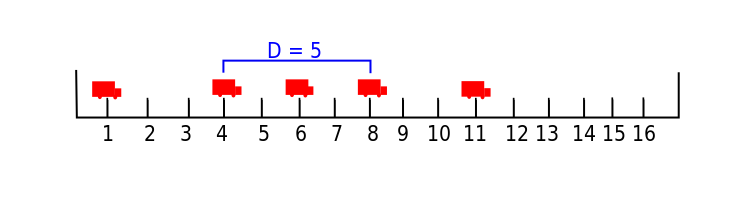
\includegraphics[scale=0.6]{images/intervalo}

\vspace{3mm}

En este caso el per\'iodo del inspector que maximiza la cantidad de camiones es el [4,8] ya que en ning\'un otro intervalo llegan m\'as de 3 camiones, por lo que esa deber\'ia ser el resultado de nuestro algoritmo.

\subsection{Funcionamiento del algoritmo}

\hspace{2mm}

En esta secci\'on daremos una idea informal acerca del funcionamiento de nuestro algoritmo para luego dar paso a las demostraciones formales.

\vspace{2mm}

\subsubsection{Preliminares}

\vspace{2mm}

La entrada del algoritmo es de la forma $D$ $n$ $d1$ $d2$ . . .$dn$, donde $D$ son los d\'ias de contrataci\'on del experto, $n$ la cantidad de camiones, y $d1$, $d2$... $dn$ los d\'ias en los que pasa cada cami\'on, no necesariamente en orden cronol\'ogico.

\vspace{2mm}

Paso 1: El algoritmo ordena los d\'ias en los que vienen los camiones de manera de tener un vector calendario. Este vector de enteros va a representar una sucesi\'on de d\'ias en los que viene al menos un cami\'on. En caso de venir m\'as de un cami\'on el mismo d\'ia, ese d\'ia aparecer\'a tantas veces como camiones vengan.

\vspace{2mm}

\vspace{2mm}

Paso 2: Una vez hecho esto, el algoritmo transforma este vector de d\'ias en un vector de tuplas$<$d\'ia, $\sharp$camiones$>$, donde $\sharp$camiones es la suma acumulada de camiones que llegaron desde el d\'ia 1 hasta ese d\'ia inclusive. De esta forma, se agrupan los d\'ias repetidos, posibilitando las b\'usquedas binarias en el vector, y al tener las sumas acumuladas hasta cada d\'ia, se puede obtener en tiempo constante la cantidad de camiones que llegaron en un intervalo [$a$..$b$], restando la suma acumulada del d\'ia anterior a $a$ a la del d\'ia $b$.

\vspace{2mm}

\subsubsection{Ciclo Principal}

\vspace{2mm}

Antes de seguir, consideremos otro caso posible del problema, en el que hay varios posibles intervalos \'optimos que maximicen la cantidad de camiones.
\{$n$ $=$ 5, d\'ias = 5,1,8,7,6; $D$ $=$ 5\}

\vspace{2mm}

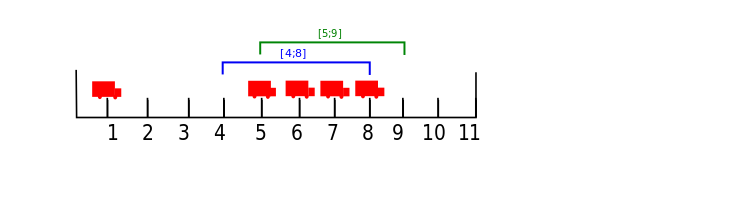
\includegraphics[scale=0.75]{images/intervalo2}

\vspace{2mm}

Vemos que en este caso hay dos intervalos que maximizan la cantidad de camiones (4): [4,8]; [5,9], llam\'mosles $a$ y $b$.

\vspace{2mm}

Seg\'un el enunciado en caso de haber varias soluciones \'optimas debemos devolver cualquiera de ellas. El funcionamiento de nuestro algoritmo hace que devuelva una particular.
Podemos ver que en el intervalo $a$, el primer cami\'on llega el d\'ia 5. Con lo cual el experto es contratado el d\'ia 4 innecesariamente, ya que no llega ning\'un cami\'on ese d\'ia. Si contrat\'aramos al experto el d\'ia 5, podr\'ia revisar todos los mismos camiones que revisaba el intervalo $a$ y tendr\'ia un d\'ia m\'as (el d\'ia 9) para revisar camiones (aunque en este caso no venga ninguno m\'as).

\vspace{2mm}

Siguiendo la l\'inea de pensamiento, cualquier intervalo \'optimo que maximice la cantidad de camiones, puede ser desplazado hacia la derecha de modo que el primer d\'ia en que es contratado el experto sea el primer d\'ia en el que viene un cami\'on en el intervalo original. Todos los camiones que abarcaba el intervalo original van a ser abarcados por el intervalo desplazado, y todos los d\'ias del principio que no eran aprovechados pasan a ser parte del final del intervalo, dando la posibilidad de poder revisar m\'as camiones. 
Por lo cual nuestro algoritmo ni siquiera considerar\'ia la evaluaci\'on del intervalo $a$ y devolver\'ia como resultado el intervalo $b$.


\vspace{2mm}

Esto es clave para entender el funcionamiento y por lo tanto la correctitud de nuestro algoritmo, ya que \'este se limita a considerar el subconjunto de intervalos de longitud $D$ que comienzan en un d\'ia en el que viene un cami\'on. El cardinal de este subconjunto, y por lo tanto la cantidad de intervalos que tiene que evaluar es n.


\vspace{2mm}

 Paso 3: La evaluaci\'on de cada intervalo se produce de la siguiente forma: En cada iteraci\'on, se toma una de las tuplas$<$dia, $\sharp camiones>$, llam\'emosle $i$. La primer componente de la tupla ($i_1$)  es el d\'ia en el que comienza el intervalo. A ese d\'ia, se le suma $D$- $1$. Este n\'umero es \'ultimo d\'ia que el experto revisa, llam\'emosle $f$. 
 
 \vspace{2mm}

Paso 4: A continuaci\'on se realiza una b\'usqueda binaria en el vector para poder obtener la suma acumulada de camiones hasta el d\'ia f. En caso de no existir este d\'ia en el vector se toma la tupla cuyo d\'ia es el menor m\'as cercano a f (Ya que no vienen camiones entre este d\'ia y $f$, la suma acumulada de camiones hasta el d\'ia menor m\'as cercano es igual a la de $f$).
\vspace{2mm}

Paso 5: Una vez obtenida la segunda tupla, se realiza la resta de: la suma acumulada hasta $f$ - la suma acumulada hasta el d\'ia $i$ -1. Esto nos da como resultado la cantidad de camiones que llegan en el intervalo [$i_1$ .. $f$], o en otras palabras la cantidad de camiones que revisa el experto si es contratado desde el dia $i_1$ hasta el $f$. Lo cual es lo que tenemos que maximizar.

\vspace{2mm}

Paso 6: Este resultado se guarda en una variable que se va reemplazando a medida que se itera por cada una de las $n$ tuplas, de forma de encontrar el m\'aximo.

\vspace{2mm}

A continuaci\'on se muestra un pseudoc\'odigo de lo anteriormente explicado.

\vspace{20mm}


\begin{algorithmic}[1]
	
	\Statex
	\Procedure{maximizarCamiones}{int diasInspector, int[] tablaDiaCantidad, int $\sharp$camiones}
	\State $Ordenar (tablaDiaCantidad)$
	\Comment{Paso 1}
	\State $AgruparYAcumular (tablaDiaCantidad)$
	\Comment{Paso 2}
	\State $int \:  maximo \gets -1$
	\State $int \: diaAContratar \gets -1$
	\For{$i \gets 0; i < tablaDiaCantidad.size; i++$}
	\Comment{Ciclo Principal}
		\State $tupla<int, \,int> \, inicio \gets tablaDiaCantidad[i]$
		\Comment{Paso 3}
		\State $int \: diaFinal \gets inicio.first + diasInspector -1$
		\State $tupla<int, int> final \gets tDC[BusquedaBinaria(tDC,i, diaFinal, tDC.size())]$
		\Comment{Paso 4}
		\State $int \sharp camionesDelIntervalo \gets final.second - tablaDiaCantidad[i-1].second$
		\Comment{Paso 5}
		\If{$\sharp camionesDelIntervalo > maximo$}
		\Comment{Paso 6}
			\State $maximo \gets camionesDelIntervalo$
			\State $diaAContratar \gets inicio.first$
		\EndIf
	\EndFor
	\State $return <diaAContratar, \, maximo>$
	\EndProcedure
	\Statex
	\end{algorithmic}

Nota: en el paso 4 abreviamos tablaDiaCantidad por tDC para una mejor lectura.

Se puede ver una implementaci\'on del algoritmo en la secci\'on \ref{codigo_1}.

\subsection{Demostraci\'on de correctitud}

Definamos algunos conceptos:

\vspace{2mm}

El algoritmo recibe $n$ naturales, con posibilidad de repetidos, que representan los d\'ias en los que llegan los camiones. Podemos representar formalmente esto con un multiconjunto de naturales, implementado con un vector al que llamaremos $calendario$. Por cada d\'ia, vienen tantos camiones como cantidad de repeticiones tenga en el multiconjunto.

\vspace{2mm}

Podemos definir formalmente las funciones $"cantCamionesDia"$, que dado un vector calendario y un dia devuelve la cantidad de camiones que llega ese d\'ia y $"cantCamionesIntervalo"$ que dado un calendario y dos d\'ias devuelve la cantidad de camiones que llegan entre esos d\'ias.

\begin{align*}
cantCamionesDia(calendario, dia) = cantRepeticiones(calendario, dia) 
\end{align*}

Donde cantRepeticiones es una funci\'on can\'onica de los multiconjuntos que dado un natural y un multiconjunto devuelve su cantidad de apariciones en \'el.

\vspace{2mm}

Definimos intervalo a un par de naturales $<x,y>$ con $x$ $\leq y$.

\begin{align*}
cantCamionesIntervalo(calendario, intervalo) = \sum_{i=intervalo_1}^{intervalo_2}( cantRepeticiones(calendario, i) ) 
\end{align*}

Esto representa la 'cantidad de camiones que llega en un intervalo'. Finalmente definamos la funci\'on principal $maximizarCamiones$, que es la formalizaci\'on matem\'atica del algoritmo. Los par\'ametros de la funci\'on son: el calendario y los d\'as que se contrata el inspector. Llamemos $I_D$ a todos los intervalos posibles entre $1$ y $max(calendario)$ de longitud D. N\'otese que al ser naturales este es un conjunto finito.

\begin{align*}
\begin{split}
maximizarCamiones(calendario, D)  =  i \in I_D / \forall x in I_D, cantCamionesIntervalo(calendario,x)& \leq  \\ cantCamionesIntervalo(i)
\end{split}
\end{align*}

\subsubsection{Correctitud de la acumulaci\'on}

Nuestro algoritmo manipula los d\'ias entrada, primero orden\'andola (la correctitud de esto est\'a asegurada por la documentaci\'on del lenguaje) y luego la transforma en un vector de tuplas, cuyas primeras componentes son los d\'ias anteriormente mencionados y las segundas componentes son la suma acumulada de camiones que llegan desde el d\'ia 1 hasta el d\'ia respectivo de su primera componente. Necesitamos probar que esta acumulaci\'on se realiza de manera correcta.

 \vspace{2mm}

Definamos formalmente la funci\'on $acumDias$ que toma un calendario y un d\'ia $d$ y devuelve la suma acumulada de camiones que llegaron desde el d\'ia 1 hasta $d$.

\begin{align*}
acumDias(calendario, dia) = \sum_{i=1}^{dia}(cantCamionesDia(calendario, i))
\end{align*}


Definido esto, vemos que podemos calcular la cantidad de camiones de un intervalo $<x, y>$ haciendo la resta:
\begin{align*}
acumDias(calendario, y) - acumDias(calendario, x-1)
\end{align*}

Probemos esto. Por definici\'on de $acumDias$:

\begin{align*}
 acumDias(calendario, y) -  acumDias(calendario,  x-1) =  \sum_{i=1}^{y}&(cantCamionesDia(calendario, i) -\\ \sum_{j=1}^{x-1}(cantCamionesDia(calendario, j)
\end{align*}
		Dado que es un intervalo, $ x \leq $ entonces:

\begin{align*}
\sum_{i=1}^{y}(cantCamionesDia(calendario, i) = \sum_{i=1}^{x-1}(cantCamiones&Dia(calendario, i) + \\ \sum_{i=x}^{y}(cantCamionesDia(calendario, i)
\end{align*}


 Si reeemplazamos en la anterior ecuaci\'on, nos queda que:


\begin{align*}
 acumDias(calendario, y) -  acumDias(calendario, x-1) = &\\  \sum_{i=1}^{x-1}(cantCamionesDia(calendario, i) + \\ \sum_{i=x}^{y}(cantCamionesDia(calendario, i)  - \\\sum_{j=1}^{x-1}(cantCamionesDia(calendario, j)
\end{align*}


Cancelando, nos queda:

\vspace{3mm}
\begin{align*}
\sum_{i=x}^{y}(cantCamionesDia(calendario, i) = cantCamionesIntervalo(calendario, <x, y>)
\end{align*}
\vspace{3mm}

Por definici\'on de $cantCamionesIntervalo$.

\vspace{2mm}



Ahora nos queda probar que nuestro algoritmo calcula correctamente la acumulaci\'on durante el ciclo. Veamos el c\'odigo.

\vspace{4mm}


\begin{algorithmic}[1]
	
	\Statex
	\Procedure{agruparYAcumular}{int entrada[]}	
	\State$vector<pair<int, int> > \: tablaDiaCantidad;$
	\State$int \: longuitud = entrada.size();$
	\State$tablaDiaCantidad.reserve(longuitud)$
	\State$int \: i=0;$
	\State$int \: acumulador = 0;$
	\While{$i < longuitud$}
		\State $acumulador++;$
		\If{$(entrada[i] != entrada[i+1]) || (i==longuitud-1)$}
			\State $pair<int, int> par = make\_pair(entrada[i], acumulador);$
			\State $tablaDiaCantidad.push\_back(par);$
		\EndIf
		\State$i++;$
	\EndWhile
	\EndProcedure
	\Statex
	\end{algorithmic}



\vspace{4mm}

El algoritmo reserva el vector de tuplas. Paso seguido declara el indice $i$ para iterar hasta $entrada.size()$ con lo cual vemos que itera sobre todos los d\'ias. Se declara el entero $acumulador$ para guardar la suma acumulada de los d\'ias en el vector.

\vspace{4mm}

Veamos el ciclo. El invariante del ciclo que tenemos es que, en cada iteraci\'on, $acumulador = \sum_{j=1}^{i-1}(cantRepeticiones(entrada[0..i), entrada[j])) $, es decir contiene la cantidad de apariciones en el vector de entrada de todos los d\'as hasta el que estamos iterando, y  $ \forall x \in entrada[0..\phi(entrada[i])] \exists y \in tablaDiaCantidad, y_1 = x \land y_2 = \sum_{j=1}^{x}(cantCamionesDia(entrada, j) \land ordenado(tablaDiaCantidad) $ , es decir, en cada iteracion, por cada d\'ia que est\'e en entrada hasta el anterior d\'ia a $i$ en el que viene un cami\'on (la funcion $\phi$ devuelve el \'indice anterior a la primera aparici\'on de entrada[i]) tablaDiaCantidad va a tener una tupla, con ese d\'ia como primer componente y la acumulaci\'ion de camiones que llegaron como segunda componente, y est\'a ordenado.

\vspace{4mm}

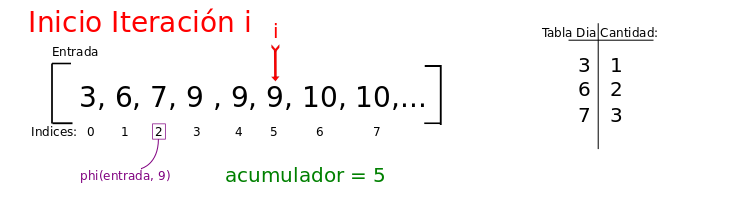
\includegraphics[scale=0.6]{images/iteracioni}

\vspace{4mm}

Suponemos que vale el invariante al comenzar el ciclo. En (7) se le suma 1 a acumulador. Podemos ver que en caso de no valer la guarda del if, no se realizan modificaciones a tablaDiaCantidad, y al final del ciclo (12) se le suma 1 a i. Por lo cual esto valida a acumulador (que suma 1 m\'as al igual que el \'indice), y se reestablece la segunda parte del invariante, al ser $entrada[i] = entrada[i+1]$, la funci\'on $\phi$ va a devolver el mismo n\'umero que en la iteraci\'on anterior, y tablaDiaCantidad no recibi\'o modificaciones.
\vspace{4mm}

En caso de valer la guarda del if, significa que $(entrada[i] != entrada[i+1]) || (i==longuitud-1)$. Si se da la primera condici\'on, acumulador tambi\'en vale al finalizar el ciclo ya que suma 1 junto con el \'indice. La segunda parte del invariante se reestablece, ya que se agrega la nueva tupla $<entrada[i], acumulador>$ a tablaDiaCantidad. La funci\'on $\phi$ en la pr\'oxima iteraci\'on va a devolver el valor de $i$ actual,  valiendo que $ \forall x \in entrada[0..\phi(entrada[i])]$, existe una tupla en tablaDiaCantidad, en particular para $entrada[i]$ es la que acabamos de agregar. La segunda componente de la nueva tupla va a ser igual a $acumulador = \sum_{j=1}^{i-1}(cantRepeticiones(entrada[0..i), entrada[i-1]))$ lo que es igual trivialmente a $ \sum_{j=1}^{x}(cantCamionesDia(entrada, j)$ por definici\'on de $cantCamionesDia$ y porque al estar ordenada $entrada$, no va a haber m\'as apariciones de el d\'ia de la nueva tupla en $entrada[i+1..0]$.

En caso de valer la segunda condici\'on, llegamos al elemento final de entrada por lo cual tenemos que agregarlo a tablaDiaCantidad, y al ser el elemento final ya no va a haber m\'as apariciones de \'el, por lo tanto no va a haber m\'as camiones que lleguen ese d\'ia, lo cual reestablece trivialmente los invariantes.

\vspace{4mm}

Con esto queda demostrado la correctitud del c\'alculo de este vector de tuplas, y sus propiedades.

\vspace{4mm}

\subsubsection{Correctitud de la reducci\'on del dominio}

Es necesario demostrar que la reducci\'on de los intervalos a analizar que realiza el algoritmo es correcta, es decir, que del conjunto de soluciones \'optimas del problema, nuestro algoritmo va a poder devolver efectivamente una de ellas. Nuestro algoritmo solamente eval\'u aquellos intervalos de longitud $D$ que comienzan con un d\'ia en el que viene al menos un cami\'on. Es bastante intuitivo pensar que, cualquier intervalo $<x,y>$ puede ser "mejorado" si se le realiza un "corrimiento a derecha" hasta el primer d\'ia en el que venga un cami\'on en el intervalo. De esta forma no se pierde ningun cami\'on y se abre la posibilidad de que vengan m\'as despues, ya que se aprovecha mejor la longitud del intervalo. 

\vspace{2mm}


Dicho formalmente, sea $c$ un natural tal que $ x \leq c \leq y$ y $cantCamionesDia(calendario, c) \geq 1$ y $\forall i \in [x..y], cantCamionesDia(calendario, i) \geq 1 \Rightarrow c \leq i $, entonces podemos transformar al intervalo $<x,y>$ en el intervalo $<c,c+D>$ y asegurarnos que $cantCamionesIntervalo(calendario, <x,y>) \leq  cantCamionesIntervalo(calendario, <c,c+D>)$.

\vspace{2mm}

Para demostrar que nuestro algoritmo realiza correctamente la reducci\'on del dominio, basta probar que del conjunto de intervalos de longitud D $\subset$ $I_D$ que son soluciones \'optimas, esta reducci\'on deja al menos uno (ya que se pide devolver s\'olo uno).

\vspace{2mm}

Necesitamos probar que para cualquier soluci\'on \'optima, podemos "construirnos" otra soluci\'on \'optima desplaz\'andola a la derecha tal que la cantidad de camiones que lleguen en los dos intervalos sea la misma, y dado que el nuevo intervalo comienza en un d\'ia en el que viene el cami\'on, va a ser evaluada por nuestro algoritmo.

Sea $\alpha = <x, y>$ una soluci\'on \'optima, es decir,
\begin{align*}
 cantCamionesIntervalo(calendario, \alpha) = maximizarCamiones(calendario, D) \land y - x = D
 \end{align*}
 Sea $c$ el natural antes descripto. Sea $\beta = <c, c+D>$. Como $\forall i \in [x..y], cantCamionesDia(calendario, i) \geq 1 \Rightarrow c \leq i $ entonces $i \in [c..c+D]$, ya que por transitividad  $x \leq c \leq i \leq y \leq c + D$. Esto se traduce a que todo d\'ia i del intervalo $\alpha$ en el que viene un cami\'on est\'a pertenece al el intervalo $\beta$. 

 \vspace{2mm}

 Como demostramos que dada una soluci\'on \'optima cualquiera podemos construirnos otra tal que pase la misma cantidad de camiones y comience en un d\'ia en el que viene uno, falta demostrar que nuestro algoritmo efectivamente eval\'ua todos los intervalos posibles que comienzan en un d\'ia en el que viene un cami\'on. Podemos verificar esto trivialmente viendo esta porci\'on del ciclo principal c\'odigo fuente.

 
\begin{algorithmic}[1]
	
	\Statex
		
	\State$for (int i = 0; i < tablaDiaCantidad.size(); ++i)$

		\State $ \: \: \: \: \: \: \: \: \:pair <int, \,int> \, target = tablaDiaCantidad[i]$
		
	


	\Statex
	\end{algorithmic}



	

  \vspace{2mm}

  Vemos que el ciclo itera de 0 a la longitud del vector de tuplas, es decir, eval\'ua todos los intervalos por los que pasa un cami\'on. 


\vspace{4mm}

\subsubsection{Correctitud del c\'alculo de los camiones de un intervalo}

Vamos a demostrar ahora que efectivamente el c\'alculo de la cantidad de camiones en un intervalo dado es correcta. Para calcularla, nuestro algoritmo realiza la resta antes propuesta: $acumDias(calendario, intervalo_1) - acumDias(calendario, intervalo_2 -1) = $

\vspace{4mm}

 Veamos la secci\'ion del ciclo principal del c\'odigo que se encarga de realizar esta tarea. Realizaremos la demostraci\'on sobre el pseudoc\'odigo para abstraernos de los iteradores y dem\'as inconveniencias del c\'odigo fuente, pero es f\'acil comprobar que ambos c\'odigos son equivalentes. 
 \vspace{2mm}


\begin{algorithmic}[1]
	
	\State $tupla<int, \,int> \, inicio \gets dias[i]$
	\State $int \: diaFinal \gets inicio.first + diasInspector -1$
	\State $tupla<int, \, int> final \gets dias[BusquedaBinaria(dias,i, diaFinal, dias.size())]$
	\State $int \sharp camionesDelIntervalo \gets final.second - dias[i-1]$
	
	\end{algorithmic}

	 \vspace{2mm}

Tomamos una tupla del vector, llamada $inicio$ (1). En su primer componente $inicio_1$ tenemos el inicio del intervalo que queremos evaluar. Para tomar el intervalo de longitud $D$ (diasInspector) que comienza en $inicio_1$, calculamos el final del intervalo como $ diaFinal = inicio_1 + D - 1$ (2). Ya tenemos el intervalo a evaluar. Entonces, para ser correcto, nuestro algoritmo deber\'ia calcular $acumDias(entrada,  diaFinal) - acumDias(entrada, inicio_1 -1)$.

\vspace{2mm}

En (3), el algoritmo realiza una b\'usqueda binaria sobre $dias$, buscando la tupla cuya primer componente sea $diaFinal$. De esta forma, en su segunda componente tenemos la suma acumulada de camiones hasta el dia final del intervalo y podriamos realizar la resta propuesta. La funci\'ion $BusquedaBinaria$ (upperBound) nos garantiza el \'indice del primer elemento mayor a $diaFinal$, al restarle uno, obtenemos o bien el \'indice de la tupla cuyo primer componente es $diaFinal$, o el \'indice de la tupla cuyo primer componente es el mayor n\'umero menor a $diaFinal$ en caso de \'este no existir. Llamamos a esta tupla $final$.

Finalmente (4), realizamos la resta $final_2 - dias[i-1]_2$. Gracias a la demostraci\'on anterior, esto podr\'ia traducirse como $ \sum_{k=1}^{final_1}(cantCamionesDia(entrada, k) - \sum_{j=1}^{dias[i-1]_1}(cantCamionesDia(entrada, j)$. Esto es igual a $acumDias(entrada, diaFinal) - acumDias(entrada, inicio_1)$, por los siguientes argumentos:

\vspace{4mm}

Veamos ahora que  $acumDias(entrada, diaFinal) = \sum_{k=1}^{final_1}(cantCamionesDia(entrada, k)$
\vspace{4mm}

Por definici\'on $acumDias(entrada, diaFinal) = \sum_{j=1}^{diaFinal}(cantCamionesDia(entrada, j)$. Si $diaFinal$ se encontraba en el calendario, entonces la b\'usqueda binaria nos devolvi\'o el \'indice de la tupla cuya primer componente es $diaFinal$, entonces $final_1 = diaFinal$, y vale la igualdad. En caso de no existir $diaFinal$ en el calendario, la b\'usqueda nos brinda el \'indice del primer elemento mayor a $diaFinal$, a lo cual rest\'andole 1 obtenemos el  mayor n\'umero menor a $diaFinal$. Esto significa que $\forall x \in [final_1 .. diaFinal], cantCamionesDia(entrada, x) = 0$. Con lo cual podemos extender la sumatoria desde $final_1$ hasta $diaFinal$, haciendo valer la igualdad.

\vspace{2mm}

Veamos que  $acumDias(entrada, inicio_1 -1) = \sum_{k=1}^{dias[i-1]}(cantCamionesDia(entrada, k)$. Por (1), $inicio_1$ = $dias[i]_1$. En caso de existir el d\'ia anterior a $inicio_1$, entonces $inicio_1 - 1 = dias[i - 1]_1$ y vale la igualdad. En caso de no existir, $dias[i-1]_1$ es el mayor n\'umero de los menores a $inicio_1$. Esto significa que $\forall x \in [dias[i-1]_1.. inicio_1-1], cantCamionesDia(entrada, x) = 0$ con lo cual puedo extender la sumatoria hasta $inicio_1-1$ y hacer avaler la igualdad.

\vspace{2mm}

Con esto demostramos que el algoritmo calcula correctamente la funci\'on que calcula la cantidad de camiones de un intervalo.



\subsubsection{Correctitud del c\'alculo del m\'aximo}

Nos queda demostrar que es correcto el c\'alculo del m\'aximo. Veamos la secci\'on del c\'odigo que calcula esto. 
\begin{algorithmic}[1]
\Statex
	\State $int \: maximo=-1;$
	\State $int \: diaAContratar=-1;$
	\For{uint i = 0; i < dias.size(); ++i}
	    \State $pair<int, int> inicio = dias[i];$

	    \State$... procesamiento \: y \: busqueda.... $
		
		\State $int \: cantCamionesDelIntervalo = (final.second-resta;$
		\If{$cantCamionesDelIntervalo>maximo$}
			\State $maximo=cantCamionesDelIntervalo;$	
			\State $diaAContratar = dias[i].first;$
		\EndIf
	\EndFor
	\State $return \: par<diaAContratar, maximo>;$
	\Statex

	\end{algorithmic}

	Podemos ver que en cada iteraci\'on, tenemos un condicional tal que si $cantCamionesDelIntervalo>maximo$ se reemplaza el m\'aximo anterior por el nuevo y el d\'a contratar. Se itera hasta el final del arreglo, por lo que la elecci\'on del m\'aximo es correcta.


\subsection{Cota de complejidad}

Lo primero que hace nuestro algoritmo es ordenar el vector de entrada. Seg\'un la documentaci\'on del lenguaje, esto se realiza en $O(n\, log \, n)$. Acto seguido nuestra funci\'on $acumularYAcumular$ reserva un vector de longitud n ($O(n)$) y realiza n iteraciones sobre el vector de entrada, en la que puede verse que realiza todas operaciones de tiempo constante (la documentaci\'on del lenguaje nos asegura esta complejidad para $make\_pair$ y $push\_back$), por lo que el ciclo es de complejidad $O(n)$. Se declaran algunas variables (tiempo constante), y finalmente se realiza el ciclo principal, en el cual se recorre de 0 a dias.size(), realizando todas operaciones de tiempo constante excepto la $BusquedaBinaria$, cuya documentaci\'on (upperBound) nos asegura tiempo logar\'itmico. Esto nos da una complejidad de $O(dias.size() \, log \, dias.size())$. Pero dado que $dias.size() \leq n$, podemos acotar por $n$ lo que nos deja una complejidad para el algoritmo (omitiendo constantes) de $O(n\, log \, n) + O(n)+  O(n) + O(n\, log \, n) = O(n\, log \, n) $.



\section{Ejercicio 2}

\subsection{Descripci\'on del problema} \label{ej_2:descripcion}

El problema se trata de un conjunto de ciudades hubicadas a cierta distancia entre ellas, las cuales todas deben de ser provistas de gas.
Para \'esto, tenemos una cantidad $k$ de centrales distribuidoras de gas, y tuber\'ias para conectar ciudades.
Una ciudad tiene gas si hay un camino de tuber\'ias que llegue hasta una central distribuidora, es decir,
si una ciudad est\'a conectada a otra ciudad por una tuber\'ia y a su vez \'esta est\'a conectada a otra ciudad
por medio de una tuber\'ia la cual tiene una central distribuidora, entonces las 3 ciudades tienen gas.
Se pide lograr que todas las ciudades tengan gas, pero que la longitud de la tuber\'ia m\'as larga de la soluci\'on
debe ser la m\'as corta posible. La longitud de una tuber\'ia es igual a la distancia entre las 2 ciudades.

El algoritmo tiene que tener una complejidad de $O(n^2)$, con $n$ la cantidad de ciudades.

De a partir de ahora, $k$ va a ser siempre la cantidad de centrales distribuidoras disponibles, y $n$ la cantidad de ciudades.

\subsubsection{Ejemplo}

Como entrada podemos tener 6 ciudades y 2 centrales distribuidoras, como en la Figura \ref{ej_2:ej:entrada}, y la soluci\'on que se busca es como indica la Figura \ref{ej_2:ej:solucion}.

\begin{figure}[htbp]
\centering
\begin{tikzpicture}

	\draw[xshift=0.5cm, yshift=0.5cm] (-1,-1) grid (7,7);
	\draw (0,0) circle [radius=0.3];
	\draw (0,0) node {1};
	\draw (1,2) circle [radius=0.3];
	\draw (1,2) node {2};
	\draw (2,3) circle [radius=0.3];
	\draw (2,3) node {3};
	\draw (3,2) circle [radius=0.3];
	\draw (3,2) node {4};
	\draw (6,5) circle [radius=0.3];
	\draw (6,5) node {5};
	\draw (6,4) circle [radius=0.3];
	\draw (6,4) node {6};
\end{tikzpicture}

\emph{Se tienen 2 centrales disponibles}

\caption{La entrada del problema, con las 5 ciudades y la cantidad de centrales}
\label{ej_2:ej:entrada}
\end{figure}

\begin{figure}[htbp]
\centering
\begin{tikzpicture}
	\draw[xshift=0.5cm, yshift=0.5cm] (-1,-1) grid (7,7);
	\draw[fill=black] (0,0) circle [radius=0.3];
	\draw[white] node (v1) at (0,0) {1};
	\draw (1,2) circle [radius=0.3];
	\draw node (v2) at (1,2) {2};
	\draw[style=dashed] (v1) -- (v2);
	\draw (2,3) circle [radius=0.3];
	\draw node (v3) at (2,3) {3};
	\draw[style=dashed] (v2) -- (v3);
	\draw (3,2) circle [radius=0.3];
	\draw node (v4) at (3,2) {4};
	\draw[style=dashed] (v3) -- (v4);
	\draw[fill=black] (6,5) circle [radius=0.3];
	\draw[white] node (v5) at (6,5) {5};
	\draw (6,4) circle [radius=0.3];
	\draw node (v6) at (6,4) {6};
	\draw[style=dashed] (v5) -- (v6);
\end{tikzpicture}
\caption{La soluci\'on al problema de la Figura \ref{ej_2:ej:entrada}, los nodos negros son los que contienen las centrales de distribuci\'on}
\label{ej_2:ej:solucion}
\end{figure}


\subsection{Ideas para la resoluci\'on} \label{ej_2:idea}

Para la resoluci\'on del problema, se puede penzar en un \emph{grafo}, donde las ciudades son nodos y las tuber\'ias las aristas,
cada arista va a tener una distancia asociada que es la distancia entre los nodos (ciudades) que conecta.

Como cada ciudad tiene gas si hay un camino hasta una central distribuidora, entonces todas las ciudades que se conectan
a una misma central pertenecen a una misma componente conexa. Como tenemos un m\'aximo de $k$ centrales, la soluci\'on tiene que tener un m\'aximo de $k$ componentes conexas y las centrales se colocar\'an cada una en una componente conexa y en cualquier ciudad dentro de la componente conexa, ya que la distancia de las aristas dentro de una componente conexa no se ver\'a modificada si se cambia de nodo la central dentro de la misma componente conexa.

Entonces, la soluci\'on que se pide es que el grafo tenga a lo sumo $k$ componentes conexas, y que la distancia de la arista mas larga, sea la m\'as corta posible.

Una idea que se propone es comenzar con todos los nodos sueltos, sin ninguna arista conectada,
y calcular todas las distancias entre todos los nodos, es decir, calcular todas las tuber\'ias posibles con sus respectivas distancias.
Luego se ordenar\'an las aristas (tuber\'ias) de menor a mayor de acuerdo a sus longitudes.
Se calcula si la cantidad de componentes conexas es menor o igual a $k$, si es as\'i, entonces el algoritmo termina, sino coloca la tuber\'ia m\'as corta que no genere un ciclo y contin\'ua preguntando sobre la cantidad de componentes conexas e iterando sobre las aristas siguiendo el orden de menor a mayor.
Es parecido al algoritmo de \emph{Kruskal}.

Para mejorar la complejidad del algoritmo, en vez de calcular la distancia de todos las aristas e iterar sobre todas las aristas, requiriendo ordenar por peso \emph{todas} las aristas, primero creamos un \'arbol generador m\'inimo (con las aristas m\'as cortas posibles), con una idea como el algoritmo de Prim y que tenga de cota $O(n^2)$,
qued\'andonos $n - 1$ aristas, y luego, al igual que antes, se ordenan y se recorren esas $n - 1$ aristas de menor a mayor.

En la secci\'on \ref{ej_2:algoritmo} se propone un pseudoc\'odigo, en la secci\'on \ref{ej_2:ejemplo} se ver\'a un ejemplo de ejecuci\'on del algoritmo,
en la secci\'on \ref{ej_2:justificacion} se justificar\'a la correctitud, y en la secci\'on \ref{ej_2:cota} se har\'a el c\'alculo de la complejidad del algoritmo.

\subsubsection{Algoritmo} \label{ej_2:algoritmo}

\begin{algorithm}[!h]
\caption{minimizarTuberias} \label{ej_2:pseudo}
\end{algorithm}
\begin{algorithmic}[1]
	\Require \emph{centrales}: cantidad de centrales disponibles, mayor que 0
	\Require \emph{ciudades}: las ciudades con sus posiciones
	\Require \emph{n}: cantidad de ciudades en el par\'ametro \emph{ciudades}
	\Statex
	\Ensure Retorna el grafo tal que hay tanas componentes conexas como \emph{centrales}, y que la arista m\'as larga es la m\'as corta posible
	\Statex
	\Procedure{minimizarTuberias}{Entero: centrales, Array: ciudades, Entero: n}{$\to$ Grafo}
		\State Grafo g $\gets$ \Call{NuevoGrafo}{$n$} \Comment{Creo un grafo con $n$ nodos, sin aristas}
		\State $<$bool agregado, entero distancia, entero nodo$>$  nodos[n] \Comment{La distancia es desde $n$ (\'indice del array) hasta nodos[$n$].nodo}
		\State $<$nodo1, nodo2, distancia$>$ aristas[n - 1]
		\Statex
		\State nodos[0] $\gets$ $<$true, 0, 0$>$ \label{ej_2:pseudo:inicializa}
		\For{i $\gets$ 1; i $<$ n; i$++$} \label{ej_2:pseudo:distancia}
			\State nodos[i] $\gets$ $<$false, \Call{Distancia}{ciudades[i], ciudades[0]}, 0$>$
		\EndFor \label{ej_2:pseudo:fin_inicializa}
		\Statex
		\For{agregados $\gets$ 0; agregados $<$ n - 1; agregados$++$} \label{ej_2:pseudo:crea_arbol}
			\State distancia\_minima $\gets$ $\infty$
			\State nodo\_minimo $\gets$ 0
			\For{i $\gets$ 0; i $<$ n; i$++$} \Comment{Busco el nodo mas cercano al \'arbol que ya tenemos} \label{ej_2:pseudo:mas_cerca}
				\If{nodos[i].agregado = false}
					\If{nodos[i].distancia $<$ distancia\_minima}
						\State distancia\_minima $\gets$ nodos[i].distancia
						\State nodo\_minimo $\gets$ i
					\EndIf
				\EndIf
			\EndFor \label{ej_2:pseudo:fin_mas_cerca}
			\Statex
			\State nodos[nodo\_minimo].agregado $\gets$ true \label{ej_2:pseudo:nodo}
			\State aristas[agregados] $\gets$ $<$nodo\_minimo, nodo[nodo\_minimo].nodo, distancia\_minima$>$ \Comment{Agrego el nodo encontrado} \label{ej_2:pseudo:arista}
			\Statex
			\For{i $\gets$ 0; i $<$ n; i$++$} \Comment{Actualizo la distancia de los nodos no agregados a\'un} \label{ej_2:pseudo:actualiza}
				\If{nodos[i].agregado = false}
					\If{nodos[i].distancia $>$ \Call{Distancia}{ciudades[i], ciudades[nodo\_minimo]}}
						\State nodo[i].distancia $\gets$ \Call{Distancia}{ciudades[i], ciudades[nodo\_minimo}
						\State nodo[i].nodo $\gets$ nodo\_minimo
					\EndIf
				\EndIf
			\EndFor \label{ej_2:pseudo:fin_actualiza}
		\EndFor \label{ej_2:pseudo:fin_crea_arbol}
		\Statex
		\State \Call{Ordenar}{aristas} \Comment{Ordeno las aristas por la distancia} \label{ej_2:pseudo:sort}
		\Statex
		\For{componentes $\gets$ n; componentes $>$ centrales; componentes$--$} \label{ej_2:pseudo:componentes}
			\State \Call{AgregarArista}{g, aristas[n - componentes].nodo1, aristas[n - componentes].nodo2}
		\EndFor \label{ej_2:pseudo:fin_componentes}
		\State retornar $\gets$ g
	\EndProcedure
\end{algorithmic}



\subsubsection{Ejemplo de ejecuci\'on} \label{ej_2:ejemplo}

\subsection{Justificaci\'on del procedimiento} \label{ej_2:justificacion}


%El Algoritmo \ref{ej_2:pseudo} se puede dividir en 4 partes. Primero de la l\'inea \ref{ej_2:pseudo:inicializa} a \ref{ej_2:pseudo:fin_inicializa} inicializa variables,
%luego de la l\'inea \ref{ej_2:pseudo:crea_arbol} a \ref{ej_2:pseudo:fin_crea_arbol} crea un \'arbol generador que la arista de mayor peso sea la menor posible,
%en la l\'inea \ref{ej_2:pseudo:sort} se ordenan las aristas del \'arbol del paso anterior,
%y entre \ref{ej_2:pseudo:componentes} y \ref{ej_2:pseudo:fin_componentes} se busca encontrar la soluci\'on con la arista m\'as corta posible.
%
%C\'omo se explic\'o en la Secci\'on \ref{ej_2:idea}, la idea del algoritmo es buscar el \'arbol con un algoritmo como Prim y luego agregar de a una las aristas de dicho \'arbol en orden de menor peso hasta encontrar la soluci\'on al problema.
%
%Vamos a demostrar que el algoritmo genera un \'arbol generador que minimiza el peso de las aristas (Secci\'on \ref{ej_2:demo:arbol}, y que a partir de las aristas del \'arbol se genera la soluci\'on al problema:
%que haya como m\'axio $k$ componentes conexas y que las aristas sean las m\'as cortas posibles (Secci\'on \ref{ej_2:demo:solucion})
%
%\subsubsection{Obtener el \'arbol} \label{ej_2:demo:arbol}
%
%La entrada que se tiene del problema es una cantidad de ciudades ($n$ nodos), las cuales pueden ser conectadas cualquier ciudad con cualquier ciudad, por lo que la entrada es un grafo completo de $n$ nodos.
%Cada arista tiene un peso, y dicho peso es el que se quiere minimizar, pero el peso de las aristas (la longitud de la tuber\'ia) depende de los nodos que conecta, y no se requiere informaci\'on extra,
%s\'olo con los 2 nodos que conecta la arista se sabe su peso (la distancia entre los nodos)
%
%El Algoritmo \ref{ej_2:pseudo} desde la l\'inea \ref{ej_2:pseudo:inicializa} a \ref{ej_2:pseudo:fin_crea_arbol} obtiene las aristas de longitud m\'inima para obtener el \'arbol generador, colocandolas en el vector \emph{aristas}.
%
%Los pasos del algoritmo son:
%\begin{enumerate}
%	\item Agarra el primer nodo del grafo y lo agrega al \'arbol que va a generar, llamemoslo $T$ (L\'inea \ref{ej_2:pseudo:inicializa})
%	\item Calcula todas las distancias del resto de los nodos hacia el primer nodo (L\'ineas \ref{ej_2:pseudo:distancia} a \ref{ej_2:pseudo:fin_inicializa})
%	\item Recorre la lista de nodos $n - 1$ veces
%	\begin{enumerate}
%		\item Busca el nodo que no pertenezca a $T$ y que tenga la distancia m\'as chica hacia el \'arbol $T$, llamemoslo $v$ (L\'ineas \ref{ej_2:pseudo:mas_cerca} a \ref{ej_2:pseudo:fin_mas_cerca})
%		\item Agrega $v$ al \'arbol $T$ con arista que va desde $v$ hacia el nodo m\'as cercano de $v$ que ya pertenec\'ia a $T$ (L\'ineas \ref{ej_2:pseudo:nodo} y \ref{ej_2:pseudo:arista})
%		\item A los nodos que a\'un no fueron agregados a $T$, le recalcula la distancia hacia el \'arbol $T$ (L\'ineas \ref{ej_2:pseudo:actualiza} a \ref{ej_2:pseudo:fin_actualiza})
%	\end{enumerate}
%\end{enumerate}
%
%\begin{proof}[Demostraci\'on: Los pasos anteriores crean un \'arbol]
%
%El \'arbol que queremos encontrar, $T$, por definici\'on es conexo y tiene $n - 1$ aristas.
%
%El algoritmo divide los nodos en 2 grupos, los agregados a $T$ que son nodos con alguna arista que lo conecta a otro nodo, y los que faltan agregar que son nodos sueltos de grado 0 (llamemoslos $V$) ($T$ y $V$ contienen nodos diferentes), cada vez que agrega una arista, est\'a uniendo un nodo $v \in T$ con un nodo $v' \in V$, sacando $v'$ de $V$ y agreg\'andolo a $T$.
%Como siempre une con una arista con un extremo un nodo que esta en $T$ (que ya est\'a unido a otro nodo en $T$) y en el otro extremo un nodo que est\'a en $V$ y no en $T$ y no es adyacente a ning\'un nodo, entonces $T$ es conexo porque todos los nodos \'estan conectados a $T$ mediante una arista al finalizar la iteraci\'on.
%Como agrega $n - 1$ aristas (L\'inea \ref{ej_2:pseudo:arista}), entonces $T$ es un grafo conexo con $n - 1$ aristas, es decir, un \emph{\'arbol}
%\end{proof}
%
%\begin{proof}[Demostraci\'on: El \'arbol anterior tiene el menor peso]
%En cada paso en que se agrega una nueva arista con un nuevo nodo, el algoritmo busca el nodo m\'as cercano al \'arbol $T$ que se est\'a armando y actualiza las distancias hacia $T$ del resto de los nodos qued\'andose con el m\'inimo entre la distancia vieja a $T$ y la distancia hacia el nuevo nodo que se agreg\'o.
%La distancia a $T$ es el peso de la arista de menor peso que une al nodo con algun nodo de $T$.
%En el algoritmo la distancia de un nodo a $T$ comienza siendo la distancia hacia el \'unico nodo que tiene $T$.
%
%Pruebo que al agregar un nuevo nodo, la distancia a $T$ va a ser la menor entre la vieja distancia a $T$ y la distancia al nuevo nodo que se agreg\'o:
%
%Siendo $d$ la distancia entre un nodo $m$ hacia $T$, significa que hay un nodo $v$ en $T$ tal que:
%\begin{equation}
%	d = distancia(m,T) \equiv
%	(\exists v \in T) (distancia(m,v) = d \land (\forall v' \in T) d <= distancia(m,v')) \label{ej_2:demo:d}
%\end{equation}
%Al agregar un nuevo nodo $w$ a $T$, sucede que las distancias viejas no cambian:
%\begin{equation*}
%	(\forall v' \in (T - w)) d <= distancia(m,v')
%\end{equation*}
%Por lo que al agregar $w$ lo que puede pasar es que $d <= distancia(m,w)$ ( en tal caso sigue valiendo la Equaci\'on \ref{ej_2:demo:d} con $w$ agregado a $T$),
%o puede ser que $d > distancia(m,w)$, entonces en ese caso para que siga valiendo la Equaci\'on \ref{ej_2:demo:d} la distancia hacia $T$ tiene que ser la distancia desde $m$ a $w$.
%Es decir, la distancia a $T$ al agregar un nuevo nodo es la menor entre la distancia vieja y la distancia hacia el nuevo nodo.
%
%El algoritmo en cada paso tiene componentes conexas, por un lado $T$ (el \'arbol que est\'a construyendo) y por otro lado cada uno de los nodos que a\'un no est\'an en $T$.
%Pruebo que teniendo una componente conexa $T$ y varios nodos sueltos, si se agregan los nodos a $T$ en orden de menor distancia entre nodo y $T$, se tiene un \'arbol con las aristas de menor peso posible:
%
%%Sea $T$ el \'arbol ya armado y $T'$ un momento en la iteraci\'on del algoritmo mientras se arma el \'arbol, $T'$ comienza con 1 nodo, y se tiene que agregar aristas para conectarlo con los nodos que a\'un no est\'an en $T'$ para formar $T$,
%%entonces en un instante del armado del \'arbol busco el nodo que tenga la menor distancia a $T'$ (lo llamo $v$) y lo uno mediante la arista $e$ al nodo m\'as cercano dentro de $T'$ (lo llamo $w$).
%%Ahora supongo que existe un mejor \'arbol $A$ tal que llega al mismo paso que $T'$ que $v$ no est\'a en $T'$ y es el m\'as cercano (es decir, $T'$ es subgrafo de $A$ y de $T$) pero no conecto $v$ con $T'$ mediante la arista $e$ (es decir, $v$ con $w$) por lo que $v$ estar\'a conectado a otro nodo en el \'arbol $A$ (porque el \'arbol es conexo) con una arista $e'$ tal que $distancia(e') < distancia(e), e' \in A, e \in T$ haciendo que al finalizar el \'arbol $T$ no minimize la mayor distancia pero $A$ si.
%%Como en $A$, $T'$ no lo conecto con $v$, entonces se tiene que conectar a otro nodo mediante una arista $a, a \in A$. Como el nodo $e$ en $T$ se hab\'ia elegido como el nodo m\'as cercano a $T'$, entonces $a$ no es el m\'as cercano y $distancia(a) > distancia(e)$, por lo que $distancia(e') < distancia(e) < distancia(a)$, como $e \notin A$ y $a \in A$ y $e' \in A$, entonces $A$ tiene una arista ($a$) con mayor distancia que la que tiene $T$, lo que contradice la suposici\'on de que $A$ sea el que minimize la distancia en vez de $T$.
%\end{proof}
%
%\subsubsection{Soluci\'on al problema} \label{ej_2:demo:solucion}
%Teniendo ya un \'arbol $T$ que contiene las aristas m\'as cortas posible, queremos armar $S$ tal que sea la soluci\'on al problema (que contenga $k$ componentes conexas como m\'aximo y que la mayor distancia sea la menor posible).
%
%\begin{proof}
%
%Luego de armar $T$, lo que se hace es ordenar las aristas de $T$ de menor a mayor seg\'un su peso (L\'inea \ref{ej_2:pseudo:sort}) y se agregan de a 1 y en cada paso se est\'a disminuyendo en 1 la cantidad de componentes conexas (porque en el \'arbol no hay ciclos)
%hasta tener $k$ componentes conexas. Como se agregan en orden de menor peso a mayor, las aristas que no se agregaron a $S$ son todas de mayor peso que las que s\'i est\'an en $S$. Suponemos entonces que se quitase la arista de mayor peso de $S$ (llamada $v$) para que
%tener la soluci\'on $S'$ tenga como mayor peso una arista m\'as corta, como $S$ no tiene ciclos (por ser subgrafo del \'arbol $T$) entonces al quitar $v$ se aumentar\'a en 1 la cantidad de componentes conexas, haciendo que sea mayor a $k$, y como no es soluci\'on se necesitar\'a colocar otra arista que no est\'e en $S$ y que no sea $v$ (porque $v$ se sac\'o para mejorar la soluci\'on), y como todas las aristas que no est\'an en $S$ son de mayor peso que las que s\'i, entonces quidando $v$ se tiene que agregar una arista de mayor peso que $v$ a $S$, haciendo que $S'$ tenga la arista m\'as larga, m\'as larga que la que ten\'ia $S$ ($v$) (valga la redundancia), contradiciendo la suposici\'on de agregando las aristas en orden y que quitando la arista m\'as larga de $S$, se obtiene un $S'$ que es mejor soluci\'on.
%\end{proof}

\subsection{Cota de complejidad} \label{ej_2:cota}

Se analiza la complejidad de algoritmo \ref{ej_2:pseudo}, para \'esto se supone que el c\'alculo de la distancia entre ciudades (el peso de las aristas/tuber\'ias) se realiza en $O(1)$

La cantidad de nodos se representar\'a como $n$, y la cantidad de centrales como $k$.

\begin{itemize}
	\item La inicializaci\'on de unas variables se realiza de la l\'inea \ref{ej_2:pseudo:inicializa} a \ref{ej_2:pseudo:fin_inicializa}, y se realizan $n$ iteraciones calculando la distancia y guardando en un vector, quedando $O(n)$
	\item Para la creaci\'on del AGM entre las l\'ineas \ref{ej_2:pseudo:crea_arbol} a \ref{ej_2:pseudo:fin_crea_arbol} realiza $n - 1$ iteraciones
	\begin{itemize}
		\item L\'ineas \ref{ej_2:pseudo:mas_cerca} a \ref{ej_2:pseudo:fin_mas_cerca}, busca el nodo m\'as cercano, realizando $n$ iteraciones de comparaciones y asignaciones que son $O(1)$, quedandonos $O(n)$
		\item Las l\'ineas \ref{ej_2:pseudo:nodo} y \ref{ej_2:pseudo:arista} son $O(1)$
		\item La actualizaci\'on de las distancias, entre las l\'ineas \ref{ej_2:pseudo:actualiza} y \ref{ej_2:pseudo:fin_actualiza} realiza $n$ iteraciones de comparaciones y asignaciones que son $O(1)$, quedandonos $O(n)$
	\end{itemize}
	\item Ordenar las aristas en la l\'inea \ref{ej_2:pseudo:sort}, y se realizan sobre las aristas agregadas en la iteraci\'on anterior, la cual agrega $n-1$ aristas, entonces se ordenan $n - 1$ elementos. Al $n$ no estar acotado, se puede realizar con algoritmos como \emph{MergeSort} o \emph{HeapSort} en $O(n \log n)$
	\item Entre las l\'ineas \ref{ej_2:pseudo:componentes} y \ref{ej_2:pseudo:fin_componentes} se realizan $n - k$ iteraciones, implementando el grafo \emph{g} en una \emph{matriz de adyacencia}, \emph{AgregarArista} se realiza en $O(1)$, quedandonos una complejidad de $O(n - k)$. Notar que si $k > n$, no se realiza ninguna iteraci\'on.
\end{itemize}

Bajo \'este an\'alisis, la complejidad nos queda (\ref{ej_2:cota:formula})

\begin{equation}
\label{ej_2:cota:formula}
\begin{split}
O(n) + (n-1)*(O(n) + O(1) + O(n)) + O(n \log n) + O(n - k) \\
=
O(n) + O(n^2) + O(n) + O(n^2) + O(n \log n) + O(n - k) \\
=
O(2n) + O(2n^2) + O(n \log n) + O(n - k) \\
= O(n^2)
\end{split}
\end{equation}

Cumpliendo as\'i la complejidad requerida.

\subsection{Casos de prueba y resultado del programa} \label{ej_2:casos}

\subsection{Mediciones de performance} \label{ej_2:performance}

\subsection{Concluciones} \label{ej_2:concluciones}


\section{Ejercicio 3}

\subsection{Descripci\'on del problema}

La entrada consta de un tablero de $n$ x $m$ casilleros y $k=n*m$ fichas cuadradas a colocar, estando cada uno de los 4 lados de las fichas identificado con un color. Se requiere colocar la mayor cantidad de fichas posibles en el tablero, tal que si 2 fichas son adyacentes, entonces el lado del cuadrado que tienen en com\'un tiene el mismo color. Las fichas ya vienen con una orientaci\'on y no pueden ser rotadas.
Ver la imagen \ref{ej_3:ej_1} para un ejemplo de la entrada, y la imagen \ref{ej_3:ej_1_sol} para ver una soluci\'on posible donde se colocan todas las fichas.
Se pide utilizar la t\'ecnica de \emph{Backtracking}
%\footnote{\emph{Backtracking} es una t\'ecnica para recorrer sistem\'aticamente todas las posibles configuraciones de un espacio asociado a soluciones candidatos de un problema computacional.}
y elaborar podas para mejorar los tiempos de ejecuci\'on.

\begin{figure}[!hbp]
\centering
\begin{tikzpicture}
\draw (0,0) grid (3,3);

\draw[fill=green] (0 + 3.5, 0 + 0) -- (0 + 3.5, 0 + 1) -- (0 + 4, 0 + 0.5) -- cycle;
\draw[fill=yellow] (0 + 3.5, 0 + 1) -- (0 + 4.5, 0 + 1) -- (0 + 4, 0 + 0.5) -- cycle;
\draw[fill=red] (0 + 4.5, 0 + 1) -- (0 + 4.5, 0 + 0) -- (0 + 4, 0 + 0.5) -- cycle;
\draw[fill=blue] (0 + 3.5, 0 + 0) -- (0 + 4.5, 0 + 0) -- (0 + 4, 0 + 0.5) -- cycle;
\node[draw, fill=white] at (0 + 4, 0 + 0.5) {7};

\draw[fill=yellow] (1 + 3.5, 0 + 0) -- (1 + 3.5, 0 + 1) -- (1 + 4, 0 + 0.5) -- cycle;
\draw[fill=green] (1 + 3.5, 0 + 1) -- (1 + 4.5, 0 + 1) -- (1 + 4, 0 + 0.5) -- cycle;
\draw[fill=yellow] (1 + 4.5, 0 + 1) -- (1 + 4.5, 0 + 0) -- (1 + 4, 0 + 0.5) -- cycle;
\draw[fill=red] (1 + 3.5, 0 + 0) -- (1 + 4.5, 0 + 0) -- (1 + 4, 0 + 0.5) -- cycle;
\node[draw, fill=white] at (1 + 4, 0 + 0.5) {8};

\draw[fill=yellow] (2 + 3.5, 0 + 0) -- (2 + 3.5, 0 + 1) -- (2 + 4, 0 + 0.5) -- cycle;
\draw[fill=green] (2 + 3.5, 0 + 1) -- (2 + 4.5, 0 + 1) -- (2 + 4, 0 + 0.5) -- cycle;
\draw[fill=red] (2 + 4.5, 0 + 1) -- (2 + 4.5, 0 + 0) -- (2 + 4, 0 + 0.5) -- cycle;
\draw[fill=blue] (2 + 3.5, 0 + 0) -- (2 + 4.5, 0 + 0) -- (2 + 4, 0 + 0.5) -- cycle;
\node[draw, fill=white] at (2 + 4, 0 + 0.5) {9};

\draw[fill=red] (0 + 3.5, 1 + 0) -- (0 + 3.5, 1 + 1) -- (0 + 4, 1 + 0.5) -- cycle;
\draw[fill=green] (0 + 3.5, 1 + 1) -- (0 + 4.5, 1 + 1) -- (0 + 4, 1 + 0.5) -- cycle;
\draw[fill=blue] (0 + 4.5, 1 + 1) -- (0 + 4.5, 1 + 0) -- (0 + 4, 1 + 0.5) -- cycle;
\draw[fill=yellow] (0 + 3.5, 1 + 0) -- (0 + 4.5, 1 + 0) -- (0 + 4, 1 + 0.5) -- cycle;
\node[draw, fill=white] at (0 + 4, 1 + 0.5) {4};

\draw[fill=blue] (1 + 3.5, 1 + 0) -- (1 + 3.5, 1 + 1) -- (1 + 4, 1 + 0.5) -- cycle;
\draw[fill=blue] (1 + 3.5, 1 + 1) -- (1 + 4.5, 1 + 1) -- (1 + 4, 1 + 0.5) -- cycle;
\draw[fill=yellow] (1 + 4.5, 1 + 1) -- (1 + 4.5, 1 + 0) -- (1 + 4, 1 + 0.5) -- cycle;
\draw[fill=green] (1 + 3.5, 1 + 0) -- (1 + 4.5, 1 + 0) -- (1 + 4, 1 + 0.5) -- cycle;
\node[draw, fill=white] at (1 + 4, 1 + 0.5) {5};

\draw[fill=red] (2 + 3.5, 1 + 0) -- (2 + 3.5, 1 + 1) -- (2 + 4, 1 + 0.5) -- cycle;
\draw[fill=yellow] (2 + 3.5, 1 + 1) -- (2 + 4.5, 1 + 1) -- (2 + 4, 1 + 0.5) -- cycle;
\draw[fill=green] (2 + 4.5, 1 + 1) -- (2 + 4.5, 1 + 0) -- (2 + 4, 1 + 0.5) -- cycle;
\draw[fill=green] (2 + 3.5, 1 + 0) -- (2 + 4.5, 1 + 0) -- (2 + 4, 1 + 0.5) -- cycle;
\node[draw, fill=white] at (2 + 4, 1 + 0.5) {6};

\draw[fill=blue] (0 + 3.5, 2 + 0) -- (0 + 3.5, 2 + 1) -- (0 + 4, 2 + 0.5) -- cycle;
\draw[fill=red] (0 + 3.5, 2 + 1) -- (0 + 4.5, 2 + 1) -- (0 + 4, 2 + 0.5) -- cycle;
\draw[fill=blue] (0 + 4.5, 2 + 1) -- (0 + 4.5, 2 + 0) -- (0 + 4, 2 + 0.5) -- cycle;
\draw[fill=yellow] (0 + 3.5, 2 + 0) -- (0 + 4.5, 2 + 0) -- (0 + 4, 2 + 0.5) -- cycle;
\node[draw, fill=white] at (0 + 4, 2 + 0.5) {1};

\draw[fill=red] (1 + 3.5, 2 + 0) -- (1 + 3.5, 2 + 1) -- (1 + 4, 2 + 0.5) -- cycle;
\draw[fill=blue] (1 + 3.5, 2 + 1) -- (1 + 4.5, 2 + 1) -- (1 + 4, 2 + 0.5) -- cycle;
\draw[fill=green] (1 + 4.5, 2 + 1) -- (1 + 4.5, 2 + 0) -- (1 + 4, 2 + 0.5) -- cycle;
\draw[fill=red] (1 + 3.5, 2 + 0) -- (1 + 4.5, 2 + 0) -- (1 + 4, 2 + 0.5) -- cycle;
\node[draw, fill=white] at (1 + 4, 2 + 0.5) {2};

\draw[fill=yellow] (2 + 3.5, 2 + 0) -- (2 + 3.5, 2 + 1) -- (2 + 4, 2 + 0.5) -- cycle;
\draw[fill=red] (2 + 3.5, 2 + 1) -- (2 + 4.5, 2 + 1) -- (2 + 4, 2 + 0.5) -- cycle;
\draw[fill=blue] (2 + 4.5, 2 + 1) -- (2 + 4.5, 2 + 0) -- (2 + 4, 2 + 0.5) -- cycle;
\draw[fill=green] (2 + 3.5, 2 + 0) -- (2 + 4.5, 2 + 0) -- (2 + 4, 2 + 0.5) -- cycle;
\node[draw, fill=white] at (2 + 4, 2 + 0.5) {3};

\end{tikzpicture}
\caption{Un tablero de 3 x 3 con las fichas que se deben colocar en el tablero}
\label{ej_3:ej_1}
\end{figure}

\begin{figure}[!hbp]
\centering
\begin{tikzpicture}

\draw[fill=green] (1 + 0, 0 + 0) -- (1 + 0, 0 + 1) -- (1 + 0.5, 0 + 0.5) -- cycle;
\draw[fill=yellow] (1 + 0, 0 + 1) -- (1 + 1, 0 + 1) -- (1 + 0.5, 0 + 0.5) -- cycle;
\draw[fill=red] (1 + 1, 0 + 1) -- (1 + 1, 0 + 0) -- (1 + 0.5, 0 + 0.5) -- cycle;
\draw[fill=blue] (1 + 0, 0 + 0) -- (1 + 1, 0 + 0) -- (1 + 0.5, 0 + 0.5) -- cycle;
\node[draw, fill=white] at (1 + 0.5, 0 + 0.5) {7};

\draw[fill=yellow] (2 + 0, 2 + 0) -- (2 + 0, 2 + 1) -- (2 + 0.5, 2 + 0.5) -- cycle;
\draw[fill=green] (2 + 0, 2 + 1) -- (2 + 1, 2 + 1) -- (2 + 0.5, 2 + 0.5) -- cycle;
\draw[fill=yellow] (2 + 1, 2 + 1) -- (2 + 1, 2 + 0) -- (2 + 0.5, 2 + 0.5) -- cycle;
\draw[fill=red] (2 + 0, 2 + 0) -- (2 + 1, 2 + 0) -- (2 + 0.5, 2 + 0.5) -- cycle;
\node[draw, fill=white] at (2 + 0.5, 2 + 0.5) {8};

\draw[fill=yellow] (0 + 0, 1 + 0) -- (0 + 0, 1 + 1) -- (0 + 0.5, 1 + 0.5) -- cycle;
\draw[fill=green] (0 + 0, 1 + 1) -- (0 + 1, 1 + 1) -- (0 + 0.5, 1 + 0.5) -- cycle;
\draw[fill=red] (0 + 1, 1 + 1) -- (0 + 1, 1 + 0) -- (0 + 0.5, 1 + 0.5) -- cycle;
\draw[fill=blue] (0 + 0, 1 + 0) -- (0 + 1, 1 + 0) -- (0 + 0.5, 1 + 0.5) -- cycle;
\node[draw, fill=white] at (0 + 0.5, 1 + 0.5) {9};

\draw[fill=red] (1 + 0, 1 + 0) -- (1 + 0, 1 + 1) -- (1 + 0.5, 1 + 0.5) -- cycle;
\draw[fill=green] (1 + 0, 1 + 1) -- (1 + 1, 1 + 1) -- (1 + 0.5, 1 + 0.5) -- cycle;
\draw[fill=blue] (1 + 1, 1 + 1) -- (1 + 1, 1 + 0) -- (1 + 0.5, 1 + 0.5) -- cycle;
\draw[fill=yellow] (1 + 0, 1 + 0) -- (1 + 1, 1 + 0) -- (1 + 0.5, 1 + 0.5) -- cycle;
\node[draw, fill=white] at (1 + 0.5, 1 + 0.5) {4};

\draw[fill=blue] (1 + 0, 2 + 0) -- (1 + 0, 2 + 1) -- (1 + 0.5, 2 + 0.5) -- cycle;
\draw[fill=blue] (1 + 0, 2 + 1) -- (1 + 1, 2 + 1) -- (1 + 0.5, 2 + 0.5) -- cycle;
\draw[fill=yellow] (1 + 1, 2 + 1) -- (1 + 1, 2 + 0) -- (1 + 0.5, 2 + 0.5) -- cycle;
\draw[fill=green] (1 + 0, 2 + 0) -- (1 + 1, 2 + 0) -- (1 + 0.5, 2 + 0.5) -- cycle;
\node[draw, fill=white] at (1 + 0.5, 2 + 0.5) {5};

\draw[fill=red] (2 + 0, 0 + 0) -- (2 + 0, 0 + 1) -- (2 + 0.5, 0 + 0.5) -- cycle;
\draw[fill=yellow] (2 + 0, 0 + 1) -- (2 + 1, 0 + 1) -- (2 + 0.5, 0 + 0.5) -- cycle;
\draw[fill=green] (2 + 1, 0 + 1) -- (2 + 1, 0 + 0) -- (2 + 0.5, 0 + 0.5) -- cycle;
\draw[fill=green] (2 + 0, 0 + 0) -- (2 + 1, 0 + 0) -- (2 + 0.5, 0 + 0.5) -- cycle;
\node[draw, fill=white] at (2 + 0.5, 0 + 0.5) {6};

\draw[fill=blue] (2 + 0, 1 + 0) -- (2 + 0, 1 + 1) -- (2 + 0.5, 1 + 0.5) -- cycle;
\draw[fill=red] (2 + 0, 1 + 1) -- (2 + 1, 1 + 1) -- (2 + 0.5, 1 + 0.5) -- cycle;
\draw[fill=blue] (2 + 1, 1 + 1) -- (2 + 1, 1 + 0) -- (2 + 0.5, 1 + 0.5) -- cycle;
\draw[fill=yellow] (2 + 0, 1 + 0) -- (2 + 1, 1 + 0) -- (2 + 0.5, 1 + 0.5) -- cycle;
\node[draw, fill=white] at (2 + 0.5, 1 + 0.5) {1};

\draw[fill=red] (0 + 0, 0 + 0) -- (0 + 0, 0 + 1) -- (0 + 0.5, 0 + 0.5) -- cycle;
\draw[fill=blue] (0 + 0, 0 + 1) -- (0 + 1, 0 + 1) -- (0 + 0.5, 0 + 0.5) -- cycle;
\draw[fill=green] (0 + 1, 0 + 1) -- (0 + 1, 0 + 0) -- (0 + 0.5, 0 + 0.5) -- cycle;
\draw[fill=red] (0 + 0, 0 + 0) -- (0 + 1, 0 + 0) -- (0 + 0.5, 0 + 0.5) -- cycle;
\node[draw, fill=white] at (0 + 0.5, 0 + 0.5) {2};

\draw[fill=yellow] (0 + 0, 2 + 0) -- (0 + 0, 2 + 1) -- (0 + 0.5, 2 + 0.5) -- cycle;
\draw[fill=red] (0 + 0, 2 + 1) -- (0 + 1, 2 + 1) -- (0 + 0.5, 2 + 0.5) -- cycle;
\draw[fill=blue] (0 + 1, 2 + 1) -- (0 + 1, 2 + 0) -- (0 + 0.5, 2 + 0.5) -- cycle;
\draw[fill=green] (0 + 0, 2 + 0) -- (0 + 1, 2 + 0) -- (0 + 0.5, 2 + 0.5) -- cycle;
\node[draw, fill=white] at (0 + 0.5, 2 + 0.5) {3};

\end{tikzpicture}
\caption{Soluci\'on colocando todas las fichas del problema de la figura \ref{ej_3:ej_1}}
\label{ej_3:ej_1_sol}
\end{figure}



\subsection{Ideas para la resoluci\'on} \label{ej_3:idea}

Como los casilleros del tablero pueden quedar vac\'ios si no se encuentra una ficha que pueda ser colocada,
llamando $k=n*m$, $n$ y $m$ las filas y columnas del tablero, y $i$ a la cantidad de casilleros que se dejan vac\'ios, para cada $i$ se pueden elegir de $\binom{k}{i}$ formas diferentes esos $i$ casilleros a dejar vac\'ios (porque de la cantidad de casilleros totales, se eligen $i$ los cuales son indistinguibles),
y para cada $i$, nos quedan $k - i$ casilleros donde colocar fichas, las cuales s\'i son distinguibles, y se pueden colocar de $k!/i!$ formas diferentes.
Por lo tanto, la cantidad de combinaciones que se pueden hacer con el tablero incluyendo dejar casilleros libres, es (\ref{ej_3:combinaciones})
\begin{equation}
	\sum_{i=0}^{k}\binom{k}{i}\frac{k!}{i!} \label{ej_3:combinaciones}
\end{equation}
\begin{equation*}
\begin{split}
	= \sum_{i=0}^{k}\frac{k!}{i!(k-i)!}\frac{k!}{i!}\\
	= \sum_{i=0}^{k}\frac{(k!)^2}{(i!)^2(k-i)!} \\
	= (k!)^2\sum_{i=0}^{k}\frac{1}{(i!)^2(k-i)!}
\end{split}
\end{equation*}

Pero para la resoluci\'on del problema s\'olo nos interesan las combinaciones v\'alidas, la idea que se plantea es ir completando el tablero casillero a casillero, y en cada casillero intentar colocar todas las fichas tal que no hayan sido colocadas antes y que al colocarla siga siendo una combinaci\'on v\'alida (que coincidan los colores con las fichas adyacentes). As\'i se van analizando s\'olo las combinaciones v\'alidas, que ser\'an menor o igual que la cuenta anterior (\ref{ej_3:k}), y retornando la combinaci\'on que contenga la mayor cantidad de fichas colocadas.

Como el resultado ser\'a una s\'ola combinaci\'on que contenga la mayor cantdidad de fichas colocadas, se puede elaborar una \emph{poda} para descartar combinaciones a medida que se est\'an armando para no terminar de generarlas y analizarlas si se determina que aunque se sigan agregando fichas a la combinaci\'on en la que se est\'a trabajando, no podr\'a contener m\'as fichas colocadas que alguna otra combinaci\'on que ya se haya calculado.
Supongamos que se est\'a trabajando con un tablero de 3 x 3 (9 fichas), y ya se proces\'o una combinaci\'on que s\'olo se deja vac\'io un casillero (contiene 8 fichas colocadas), guardando esta posible soluci\'on como la que m\'as fichas contiene; y actualmente se est\'a procesando una posible soluci\'on que ya analiz\'o 6 casilleros del tablero (quedando 3 a\'un por procesar), pero tuvo que dejar 2 casilleros vac\'ios (es decir, de los 6 casilleros 4 contienen fichas),
si en los 3 casilleros restantes colocase 3 fichas (lo m\'aximo que puede conseguir), esta combinaci\'on tendr\'ia 7 fichas colocadas (4 que ya hab\'ia colocado mas 3 posibles fichas que puede colocar a continuaci\'on) y 2 casilleros vac\'ios, siendo menor a la candidad de 8 fichas de la soluci\'on guardad como m\'axima encontrada hasta el momento, por lo que se puede descartar la soluci\'on que se ven\'ia procesando porque nunca podr\'ia llegar a ser una soluci\'on al problema.

\subsubsection{Algoritmo para la resoluci\'on propuesta} \label{ej_3:algo}

Como se describi\'o en la secci\'on (\ref{ej_3:idea}), la resoluci\'on del problema se basa en 2 ideas, s\'olo analizar combinaciones v\'alidas y descartar combinaciones si ya se calcula que no pueden superar a una combinaci\'on m\'axima ya encontrada.
Se propone el algoritmo \ref{ej_3:pseudo}.

\begin{algorithm}
	\caption{maximizarTablero} \label{ej_3:pseudo}
\end{algorithm} %sino no divide el codigo en paginas
\begin{algorithmic}[1]
	\Require \emph{tablero}: el tablero donde se ir\'an colocando las fichas
	\Require \emph{n, m}: filas y columnas del tablero
	\Require \emph{fichas\_disponibles}: array con las fichas aun diponibles por poner
	\Require \emph{i\_actual, j\_actual}: la posici\'on que se tiene que procesar
	\Require \emph{casilleros\_calculados}: cantidad de casilleros que ya se procesaron
	\Require \emph{fichas\_colocadas}: cantidad de fichas colocadas (no se cuentan los casilleros vac\'ios dejados)
	\Require \emph{tablero\_optimo}: el optimo encontrado hasta el momento
	\Require \emph{fichas\_maximas}: cantidad m\'axima de fichas que se pudieron colocar en el tablero\_optimo
	\Ensure La funci\'on va a dejar en \emph{tablero\_optimo} y en \emph{fichas\_maximas} la mejor combinaci\'on que pudo encontrar de fichas tal que las fichas adyacentes comparten el color en el borde que tienen en com\'un, y es la combinaci\'on en la que m\'as fichas se pudo colocar
	\Statex
	\Procedure{maximizarTablero}{tablero, n, m, fichas\_disponibles, i\_actual, j\_actual, casilleros\_calculados, fichas\_colocadas, tablero\_optimo, fichas\_maximas}
	\State $total\_casilleros \gets n*m$
	\State $n\_fichas \gets total\_casilleros$
	\If{$casilleros\_calculados = total\_casilleros$} \label{ej_3:pseudo:base}
		\If{$fichas\_colocadas > fichas\_maximas$}
			\State copiarTablero(tablero\_optimo, tablero)
			\State $fichas\_maximas \gets fichas\_colocadas$
		\EndIf
		\State return
	\EndIf \label{ej_3:pseudo:base_end}
	\If{$total\_casilleros - casilleros\_calculados + fichas\_colocadas <= fichas\_maxima$} \label{ej_3:pseudo:poda}
		\State return
	\EndIf
	\State $proximo\_i \gets i\_actual$ \label{ej_3:pseudo:proximo}
	\State $proximo\_j \gets j\_actual$
	\If{$i\_actual = n - 1$}
		\State $proximo\_i \gets 0$
		\State $proximo\_j++$
	\Else
		\State $proximo\_i++$
	\EndIf \label{ej_3:pseudo:proximo_end}
	\For{$f \in fichas\_disponibles$} \label{ej_3:pseudo:fichas} \label{ej_3:pseudo:disponible}
		\If{validaColocar(f, tablero, i\_actual, j\_actual)} \label{ej_3:pseudo:valida}
			\State $tablero[i\_actual][j\_actual] = f$ \label{ej_3:pseudo:coloca}
			\If{$\neg f->vacia$} \label{ej_3:pseudo:vacia}
				\State $fichas\_nuevas \gets fichas\_disponibles - f$
				\State $fichas\_colocadas++$
			\Else
				\State $fichas\_nuevas \gets fichas\_disponibles$
			\EndIf
			\State maximizarTablero(tablero, n, m, fichas\_nuevas, i\_proximo, j\_proximo, casilleros\_calculados + 1, fichas\_colocadas, tablero\_optimo, fichas\_maximas) \label{ej_3:pseudo:recursion}
			\If{$\neg f->vacia$}
				\State $fichas\_colocadas--$
			\EndIf
		\EndIf
	\EndFor \label{ej_3:pseudo:fichas_end}
	\EndProcedure
	\Statex
	\Procedure{bool validaColocar}{ficha, tablero, i, j} \label{ej_3:pseudo:validaColocar}
		\If{$ficha->vacia$}
			\State $return \gets true$
		\EndIf
		\If{$j > 0$}
			\If{$\neg tablero[i][j - 1]->vacia$}
				\If{$tablero[i][j - 1]->derecha \neq fichas->izquierda$}
					\State $return \gets false$
				\EndIf
			\EndIf
		\EndIf
		\If{$i > 0$}
			\If{$\neg tablero[i - 1][j]->vacia$}
				\If{$tablero[i- 1][j]->abajo \neq fichas->arriba$}
					\State $return \gets false$
				\EndIf
			\EndIf
		\EndIf
		\State $return \gets true$
	\EndProcedure
\end{algorithmic}

%\begin{procedure}
%	\SetKwProg{Fn}{}{}{}
%	\SetStartEndCondition{ (}{)}{)}\SetAlgoBlockMarkers{\{}{\}}
%	\SetKwFunction{maximizarTablero}{maximizarTablero}
%	\SetKwFunction{copiarTablero}{copiarTablero}
%	\KwIn{\emph{tablero}: el tablero donde se ir\'an colocando las fichas}
%	\KwIn{\emph{n, m}: filas y columnas del tablero}
%	\KwIn{\emph{fichas\_disponibles}: array con las fichas aun diponibles por poner}
%	\KwIn{\emph{i\_actual, j\_actual}: la posici\'on que se tiene que procesar}
%	\KwIn{\emph{casilleros\_calculados}: cantidad de casilleros que ya se procesaron}
%	\KwIn{\emph{fichas\_colocadas}: cantidad de fichas colocadas (no se cuentan los casilleros vac\'ios dejados)}
%	\KwIn{\emph{tablero\_optimo}: el optimo encontrado hasta el momento}
%	\KwIn{\emph{fichas\_maximas}: cantidad m\'axima de fichas que se pudieron colocar en el tablero\_optimo}
%	\KwOut{La funci\'on va a dejar en \emph{tablero\_optimo} y en \emph{fichas\_maximas} la mejor combinaci\'on que pudo encontrar de fichas tal que las fichas adyacentes comparten el color en el borde que tienen en com\'un, y es la combinaci\'on en la que m\'as fichas se pudo colocar}
%	\Fn(){void \maximizarTablero{tablero, n, m, fichas\_disponibles, i\_actual, j\_actual, casilleros\_calculados, fichas\_colocadas, tablero\_optimo, fichas\_maximas}}{
%		$total\_casilleros \leftarrow n*m$\;
%		$n\_fichas \leftarrow total\_casilleros$\;
%		\If{$casilleros\_calculados = total\_casilleros$}{
%			\If{$fichas\_colocadas > fichas\_maximas$}{
%				\copiarTablero{tablero\_optimo, tablero}
%				$fichas\_maximas \leftarrow fichas\_colocadas$\;
%			}
%			\KwRet
%		}
%		\If{$total\_casilleros - casilleros\_calculados + fichas\_colocadas <= fichas\_maxima$}{
%			\KwRet;
%		}
%		$proximo\_i \leftarrow i\_actual$\;
%		$proximo\_j \leftarrow j\_actual$\;
%		\uIf{$j\_actual = m - 1$}{
%			$proximo\_j = 0$\;
%			$proximo\_i++$\;
%		}
%		\Else{
%			$proximo\_j++$\;
%		}
%		\For{$i \leftarrow 0; i < n\_fichas; i++$}{
%			\If{$fichas\_disponibles[i]$}{
%				\If{$fichas\_disponibles[i]->numero >= 0$}{
%					\If{$j\_actual > 0$}{
%						\If{$tablero[i\_actual][j\_actual - 1]->numero >= 0$}{
%							\If{$tablero[i\_actual][j\_actual - 1]->derecha \neq fichas\_disponibles[i]->izquierda$}{
%								$continue$\;
%							}
%						}
%					}
%					\If{$i\_actual > 0$}{
%						\If{$tablero[i\_actual - 1][j\_actual]->numero >= 0$}{
%							\If{$tablero[i\_actual - 1][j\_actual]->abajo \neq fichas\_disponibles[i]->arriba$}{
%								$continue$\;
%							}
%						}
%					}
%				}
%				$tablero[i\_actual][j\_actual] = fichas\_disponibles[i]$\;
%				\If{$fichas\_disponibles[i]->numero >= 0$}{
%					$fichas\_disponibles[i] \leftarrow NULL$\;
%					$fichas\_en\_tablero++$\;
%				}
%				$casilleros\_tablero++$\;
%				\maximizarTablero{tablero, n, m, fichas\_disponibles, i\_proximo, j\_proximo, casilleros\_calculados, fichas\_colocadas, tablero\_optimo, fichas\_maximas}
%				\If{$fichas[i].numero >= 0$}{
%					$fichas\_disponibles[i] \leftarrow \&fichas[i]$\;
%					$fichas\_en\_tablero--$\;
%				}
%				$casilleros\_tablero--$\;
%			}
%		}
%		\KwRet
%	}
%	\caption{maximizarTablero()} \label{ej_3:pseudo}
%\end{procedure}



La funci\'on maximizarTablero (algoritmo \ref{ej_3:pseudo}), es recursiva y en la primera llamada debe llamarse con \emph{tablero}, siendo una matriz de $n * m$, donde se colocar\'an las fichas.
\emph{n} y \emph{m} son las filas y columnas del \emph{tablero}.
\emph{fichas\_disponibles} tiene que contener todas las fichas que vinieron en la entrada y con el campo \emph{vac\'ia} en $false$, m\'as una ficha con el campo \emph{vac\'ia} en $true$ (para indicar que ese casillero se dejo vac\'io).
\emph{i\_actual}, \emph{j\_actual}, \emph{casilleros\_calculados} y \emph{fichas\_colocadas} tienen que estar en $0$.
\emph{tablero\_optimo} es donde se va a colocar el tablero con mayor cantidad de fichas colocadas, y en \emph{fichas\_maximas} se va a colocar la cantidad de fichas en dicho tablero, \emph{fichas\_maximas} debe estar en un valor menor a 0 cuando se llama al algoritmo.

El algoritmo (\ref{ej_3:pseudo}) lo que realiza es llamarse recursivamente probando en cada casillero todas las fichas que esten disponibles para poner y que sea valido colocarlas.

Entre las l\'ineas \ref{ej_3:pseudo:base} y \ref{ej_3:pseudo:base_end} se encuentra el caso base de la recursi\'on, el cual sucede cuando ya se procesaron todos los casilleros, si la cantidad de fichas colocadas es mayor a la cantidad m\'axima que se hab\'ia almacenado, entonces reemplaza el \emph{tablero\_optimo} con el tablero actual, y actualiza la variable \emph{fichas\_maximas}.

Luego en la l\'inea \ref{ej_3:pseudo:poda} se encuentra la \emph{poda} para cortar con la recursi\'on antes de procesar todos los casilleros si aunque se completen todos los casilleros restantes con fichas, no superar\'an la cantidad m\'axima de fichas que ya se almacen\'o con otra combinaci\'on.

Entre las l\'ineas \ref{ej_3:pseudo:proximo} y \ref{ej_3:pseudo:proximo_end} se calcula el pr\'oximo casillero que se deber\'a llamar en la recursi\'on

Y por \'ultimo entre las l\'ineas \ref{ej_3:pseudo:fichas} y \ref{ej_3:pseudo:fichas_end} se buscan todas las fichas disponibles para colocar (l\'inea \ref{ej_3:pseudo:disponible}) y que sea v\'alida su colocaci\'on (l\'inea \ref{ej_3:pseudo:valida}), entonces si se cumplen dichas condiciones,
coloca la ficha en el tablero (l\'inea \ref{ej_3:pseudo:coloca}) y si no es la ficha que corresponde al casillero vac\'io (l\'inea \ref{ej_3:pseudo:vacia}) la elmina de las fichas disponibles,
y se llama recursivamente (l\'linea \ref{ej_3:pseudo:recursion}) con la nueva posici\'on a analizar.

Tambi\'em se encuentra la funci\'on \emph{validaColocar} como una funci\'on auxiliar que retornar\'a $true$ si colocar la \emph{ficha} en el \emph{tablero} en la posici\'on \emph{i, j},
pero tiene en cuenta que el tablero se va completando de izquierda a derecha y de abajo a izquierda (el $(0; 0)$ corresponde a arriba a la izquierda), y en base a esto s\'olo chequea 2 lados de la ficha a colocar y no los 4.

En la secci\'on (\ref{ej_3:justificacion}) se hablar\'a sobre la justificaci\'on y correctitud del algoritmo.

Se puede ver una implementaci\'on del algoritmo en la secci\'on \ref{codigo_2}.

\subsubsection{Ejemplo de la resoluci\'on propuesta}
\label{ej_3:ejemplo}

Siguiendo los pasos del algoritmo de la secci\'on \ref{ej_3:algo}, se procede a un ejemplo de la ejecuci\'on con un tablero de 2 x 2 y 4 fichas, y 3 colores (imagen \ref{ej_3:entrada}, todas las im\'agenes se encuentran al final de la secci\'on \ref{ej_3:ejemplo}), agregando la ficha \emph{V} para indicar dejar el casillero vac\'io

El algoritmo comienza en la posici\'on $(0;0)$ y comienza a iterar por todas las fichas disponibles, comenzando por la n\'umero 1, la cual es v\'alida de colocar (ya que no tiene fichas al rededor) (imagen \ref{ej_3:primera}) y la coloca, llando recursivamente al algoritmo pas\'andole como posici\'on el valor $(0;1)$.

Ahora vuelve a recorrer la lista de fichas disponibles (la ficha 2, 3 y 4) y como la ficha 2 no es v\'alida de colocar (el color no coincide) (imagen \ref{ej_3:segunda}), entonces avanza a la siguiente ficha, la 3 y como es v\'alida (comparte el color verde), la coloca (imagen \ref{ej_3:segunda_valida}) y se llama recursivamente ahora con la posici\'on $(1;0)$.
Como descart\'o la ficha 2 para \'esta posici\'on con la ficha 1 colocada en la primera posici\'on, ya descart\'o todos los casos que comienzen con la ficha 1 en la posici\'on $(0;0)$ y la ficha 2 en $(0;1)$ (7 casos contando dejar casilleros vac\'ios)

Quedando 2 fichas disponibles, y estando posicionado en $(1;0)$, la primer ficha disponible es la n\'umeroro 2, la cual es v\'alida de colocar (imagen \ref{ej_3:ante_ultima}) y llama recursivamente para posicionarse en $(1;1)$ y la \'ultima ficha disponible tambi\'en es v\'alida y es colocada (imagen \ref{ej_3:ultima_ficha}).

En la siguiente llamada recursiva, ya todos los casilleros fueron procesados por ende entra en el caso base del algoritmo (\ref{ej_3:pseudo}), el cual como no ten\'ia valor cargado para la cantidad m\'axima de fichas ya calculadas, guarda \'esta opci\'on como la mejor combinaci\'on hasta el momento con 4 fichas colocadas (imagen \ref{ej_3:caso_base}).

Luego de \'esto, retorna de la recursi\'on y vuelve a quedar con un casillero sin procesar y con la ficha 4 disponible y la `ficha vac\'ia' disponible, la ficha 4 la proces\'o en la iteraci\'on anterior, por lo que intenta con la ficha vac\'ia (imagen \ref{ej_3:ficha_vacia}), llama nuevamente a la recursi\'on, pero como tiene 3 fichas colocadas en vez de 4 que se tiene guardado como mejor resultado hasta el momento, entonces retorna y descarta la combinaci\'on. Al haber procesado para el \'ultimo casillero todas las posibilidades, vuelve a retornar de la recursi\'on quedando 2 casilleros sin procesar y 2 fichas disponibles, la ficha 2 ya fue procesada por lo que intenta con la 4, la cu\'al no es v\'alida de colocar, y termina dejando el casillero vac\'io y llamar recursivamente para el \'ultimo casillero. En este caso entra en la condici\'on de la \emph{poda}, ya que tiene 2 casilleros con fichas, y queda 1 casillero por procesar, lo cual nunca podr\'a superar a las 4 fichas m\'aximas que pudo poner anteriormente.

De a partir de ahora como 4 es lo m\'aximo que se puede colocar, todas las dem\'as combinaciones que se intenten van a entrar en la condici\'on de la \emph{poda} y el algoritmo va a terminar retornando como combinaci\'on \'optima el tablero guardado de la imagen \ref{ej_3:caso_base}

\begin{figure}[!htbp]
\centering
\begin{tikzpicture}

\draw (0,0) grid (2,2);

\draw[fill=red] (0 + 2.5, 0 + 2) -- (0 + 3.5, 0 + 2) -- (0 + 3, 0 + 1.5) -- cycle;
\draw[fill=green] (0 + 2.5, 0 + 2) -- (0 + 2.5, 0 + 1) -- (0 + 3, 0 + 1.5) -- cycle;
\draw[fill=blue] (0 + 2.5, 0 + 1) -- (0 + 3.5, 0 + 1) -- (0 + 3, 0 + 1.5) -- cycle;
\draw[fill=green] (0 + 3.5, 0 + 1) -- (0 + 3.5, 0 + 2) -- (0 + 3, 0 + 1.5) -- cycle;
\node[draw, fill=white] at (0 + 3, 0 + 1.5) {1};

\draw[fill=blue] (1 + 2.5, 0 + 2) -- (1 + 3.5, 0 + 2) -- (1 + 3, 0 + 1.5) -- cycle;
\draw[fill=blue] (1 + 2.5, 0 + 2) -- (1 + 2.5, 0 + 1) -- (1 + 3, 0 + 1.5) -- cycle;
\draw[fill=red] (1 + 2.5, 0 + 1) -- (1 + 3.5, 0 + 1) -- (1 + 3, 0 + 1.5) -- cycle;
\draw[fill=green] (1 + 3.5, 0 + 1) -- (1 + 3.5, 0 + 2) -- (1 + 3, 0 + 1.5) -- cycle;
\node[draw, fill=white] at (1 + 3, 0 + 1.5) {2};

\draw[fill=blue] (2 + 2.5, 0 + 2) -- (2 + 3.5, 0 + 2) -- (2 + 3, 0 + 1.5) -- cycle;
\draw[fill=green] (2 + 2.5, 0 + 2) -- (2 + 2.5, 0 + 1) -- (2 + 3, 0 + 1.5) -- cycle;
\draw[fill=red] (2 + 2.5, 0 + 1) -- (2 + 3.5, 0 + 1) -- (2 + 3, 0 + 1.5) -- cycle;
\draw[fill=blue] (2 + 3.5, 0 + 1) -- (2 + 3.5, 0 + 2) -- (2 + 3, 0 + 1.5) -- cycle;
\node[draw, fill=white] at (2 + 3, 0 + 1.5) {3};

\draw[fill=red] (3 + 2.5, 0 + 2) -- (3 + 3.5, 0 + 2) -- (3 + 3, 0 + 1.5) -- cycle;
\draw[fill=green] (3 + 2.5, 0 + 2) -- (3 + 2.5, 0 + 1) -- (3 + 3, 0 + 1.5) -- cycle;
\draw[fill=red] (3 + 2.5, 0 + 1) -- (3 + 3.5, 0 + 1) -- (3 + 3, 0 + 1.5) -- cycle;
\draw[fill=green] (3 + 3.5, 0 + 1) -- (3 + 3.5, 0 + 2) -- (3 + 3, 0 + 1.5) -- cycle;
\node[draw, fill=white] at (3 + 3, 0 + 1.5) {4};

\draw[black] (4 + 2.5, 0 + 2) rectangle (5 + 2.5, 1);
\node[draw, fill=white] at (4 + 3, 0 + 1.5) {V};

\end{tikzpicture}

\caption{Tablero y fichas de entrada. La ficha \emph{V} va a representar dejar el casillero vac\'io}
\label{ej_3:entrada}
\end{figure}

\begin{figure}[!htbp]
\centering
\begin{tikzpicture}

\draw (0,0) grid (2,2);

\draw[brown,very thick] (0,2) rectangle (1,1);

\draw[brown,very thick,fill=red] (0 + 2.5, 0 + 2) -- (0 + 3.5, 0 + 2) -- (0 + 3, 0 + 1.5) -- cycle;
\draw[brown,very thick,fill=green] (0 + 2.5, 0 + 2) -- (0 + 2.5, 0 + 1) -- (0 + 3, 0 + 1.5) -- cycle;
\draw[brown,very thick,fill=blue] (0 + 2.5, 0 + 1) -- (0 + 3.5, 0 + 1) -- (0 + 3, 0 + 1.5) -- cycle;
\draw[brown,very thick,fill=green] (0 + 3.5, 0 + 1) -- (0 + 3.5, 0 + 2) -- (0 + 3, 0 + 1.5) -- cycle;
\node[draw, fill=white] at (0 + 3, 0 + 1.5) {1};

\draw[->,thick] (0 + 3, 0 + 1.5) -- (0 + 0.5, 0 + 1.5);

\draw[fill=blue] (1 + 2.5, 0 + 2) -- (1 + 3.5, 0 + 2) -- (1 + 3, 0 + 1.5) -- cycle;
\draw[fill=blue] (1 + 2.5, 0 + 2) -- (1 + 2.5, 0 + 1) -- (1 + 3, 0 + 1.5) -- cycle;
\draw[fill=red] (1 + 2.5, 0 + 1) -- (1 + 3.5, 0 + 1) -- (1 + 3, 0 + 1.5) -- cycle;
\draw[fill=green] (1 + 3.5, 0 + 1) -- (1 + 3.5, 0 + 2) -- (1 + 3, 0 + 1.5) -- cycle;
\node[draw, fill=white] at (1 + 3, 0 + 1.5) {2};

\draw[fill=blue] (2 + 2.5, 0 + 2) -- (2 + 3.5, 0 + 2) -- (2 + 3, 0 + 1.5) -- cycle;
\draw[fill=green] (2 + 2.5, 0 + 2) -- (2 + 2.5, 0 + 1) -- (2 + 3, 0 + 1.5) -- cycle;
\draw[fill=red] (2 + 2.5, 0 + 1) -- (2 + 3.5, 0 + 1) -- (2 + 3, 0 + 1.5) -- cycle;
\draw[fill=blue] (2 + 3.5, 0 + 1) -- (2 + 3.5, 0 + 2) -- (2 + 3, 0 + 1.5) -- cycle;
\node[draw, fill=white] at (2 + 3, 0 + 1.5) {3};

\draw[fill=red] (3 + 2.5, 0 + 2) -- (3 + 3.5, 0 + 2) -- (3 + 3, 0 + 1.5) -- cycle;
\draw[fill=green] (3 + 2.5, 0 + 2) -- (3 + 2.5, 0 + 1) -- (3 + 3, 0 + 1.5) -- cycle;
\draw[fill=red] (3 + 2.5, 0 + 1) -- (3 + 3.5, 0 + 1) -- (3 + 3, 0 + 1.5) -- cycle;
\draw[fill=green] (3 + 3.5, 0 + 1) -- (3 + 3.5, 0 + 2) -- (3 + 3, 0 + 1.5) -- cycle;
\node[draw, fill=white] at (3 + 3, 0 + 1.5) {4};

\draw[black] (4 + 2.5, 0 + 2) rectangle (5 + 2.5, 1);
\node[draw, fill=white] at (4 + 3, 0 + 1.5) {V};

\end{tikzpicture}

\caption{Comienza con la primer posici\'on del tablero y la primera ficha disponible para colocar, siendo esta v\'alida para ser colocada}
\label{ej_3:primera}
\end{figure}

\begin{figure}[!htbp]
\centering
\begin{tikzpicture}

\draw (0,0) grid (2,2);

\draw[brown,very thick] (1,2) rectangle (2,1);

\draw[fill=red] (0 + 0, 0 + 2) -- (0 + 1, 0 + 2) -- (0 + 0.5, 0 + 1.5) -- cycle;
\draw[fill=green] (0 + 0, 0 + 2) -- (0 + 0, 0 + 1) -- (0 + 0.5, 0 + 1.5) -- cycle;
\draw[fill=blue] (0 + 0, 0 + 1) -- (0 + 1, 0 + 1) -- (0 + 0.5, 0 + 1.5) -- cycle;
\draw[fill=green] (0 + 1, 0 + 1) -- (0 + 1, 0 + 2) -- (0 + 0.5, 0 + 1.5) -- cycle;
\node[draw, fill=white] at (0 + 0.5, 0 + 1.5) {1};

\draw[brown,very thick,fill=blue] (1 + 2.5, 0 + 2) -- (1 + 3.5, 0 + 2) -- (1 + 3, 0 + 1.5) -- cycle;
\draw[brown,very thick,fill=blue] (1 + 2.5, 0 + 2) -- (1 + 2.5, 0 + 1) -- (1 + 3, 0 + 1.5) -- cycle;
\draw[brown,very thick,fill=red] (1 + 2.5, 0 + 1) -- (1 + 3.5, 0 + 1) -- (1 + 3, 0 + 1.5) -- cycle;
\draw[brown,very thick,fill=green] (1 + 3.5, 0 + 1) -- (1 + 3.5, 0 + 2) -- (1 + 3, 0 + 1.5) -- cycle;
\node[draw, fill=white] at (1 + 3, 0 + 1.5) {2};

\draw[fill=blue] (2 + 2.5, 0 + 2) -- (2 + 3.5, 0 + 2) -- (2 + 3, 0 + 1.5) -- cycle;
\draw[fill=green] (2 + 2.5, 0 + 2) -- (2 + 2.5, 0 + 1) -- (2 + 3, 0 + 1.5) -- cycle;
\draw[fill=red] (2 + 2.5, 0 + 1) -- (2 + 3.5, 0 + 1) -- (2 + 3, 0 + 1.5) -- cycle;
\draw[fill=blue] (2 + 3.5, 0 + 1) -- (2 + 3.5, 0 + 2) -- (2 + 3, 0 + 1.5) -- cycle;
\node[draw, fill=white] at (2 + 3, 0 + 1.5) {3};

\draw[fill=red] (3 + 2.5, 0 + 2) -- (3 + 3.5, 0 + 2) -- (3 + 3, 0 + 1.5) -- cycle;
\draw[fill=green] (3 + 2.5, 0 + 2) -- (3 + 2.5, 0 + 1) -- (3 + 3, 0 + 1.5) -- cycle;
\draw[fill=red] (3 + 2.5, 0 + 1) -- (3 + 3.5, 0 + 1) -- (3 + 3, 0 + 1.5) -- cycle;
\draw[fill=green] (3 + 3.5, 0 + 1) -- (3 + 3.5, 0 + 2) -- (3 + 3, 0 + 1.5) -- cycle;
\node[draw, fill=white] at (3 + 3, 0 + 1.5) {4};

\draw[black] (4 + 2.5, 0 + 2) rectangle (5 + 2.5, 1);
\node[draw, fill=white] at (4 + 3, 0 + 1.5) {V};

\end{tikzpicture}

\caption{Se mueve a la segunda posici\'on el tablero y analiza la primer ficha disponible, pero no es v\'alida su colocaci\'on}
\label{ej_3:segunda}
\end{figure}

\begin{figure}[!htbp]
\centering
\begin{tikzpicture}

\draw (0,0) grid (2,2);

\draw[brown,very thick] (1,2) rectangle (2,1);

\draw[fill=red] (0 + 0, 0 + 2) -- (0 + 1, 0 + 2) -- (0 + 0.5, 0 + 1.5) -- cycle;
\draw[fill=green] (0 + 0, 0 + 2) -- (0 + 0, 0 + 1) -- (0 + 0.5, 0 + 1.5) -- cycle;
\draw[fill=blue] (0 + 0, 0 + 1) -- (0 + 1, 0 + 1) -- (0 + 0.5, 0 + 1.5) -- cycle;
\draw[fill=green] (0 + 1, 0 + 1) -- (0 + 1, 0 + 2) -- (0 + 0.5, 0 + 1.5) -- cycle;
\node[draw, fill=white] at (0 + 0.5, 0 + 1.5) {1};

\draw[fill=blue] (1 + 2.5, 0 + 2) -- (1 + 3.5, 0 + 2) -- (1 + 3, 0 + 1.5) -- cycle;
\draw[fill=blue] (1 + 2.5, 0 + 2) -- (1 + 2.5, 0 + 1) -- (1 + 3, 0 + 1.5) -- cycle;
\draw[fill=red] (1 + 2.5, 0 + 1) -- (1 + 3.5, 0 + 1) -- (1 + 3, 0 + 1.5) -- cycle;
\draw[fill=green] (1 + 3.5, 0 + 1) -- (1 + 3.5, 0 + 2) -- (1 + 3, 0 + 1.5) -- cycle;
\node[draw, fill=white] at (1 + 3, 0 + 1.5) {2};

\draw[brown,very thick,fill=blue] (2 + 2.5, 0 + 2) -- (2 + 3.5, 0 + 2) -- (2 + 3, 0 + 1.5) -- cycle;
\draw[brown,very thick,fill=green] (2 + 2.5, 0 + 2) -- (2 + 2.5, 0 + 1) -- (2 + 3, 0 + 1.5) -- cycle;
\draw[brown,very thick,fill=red] (2 + 2.5, 0 + 1) -- (2 + 3.5, 0 + 1) -- (2 + 3, 0 + 1.5) -- cycle;
\draw[brown,very thick,fill=blue] (2 + 3.5, 0 + 1) -- (2 + 3.5, 0 + 2) -- (2 + 3, 0 + 1.5) -- cycle;
\node[draw, fill=white] at (2 + 3, 0 + 1.5) {3};

\draw[->,thick] (0 + 5, 0 + 1.5) -- (0 + 1.5, 0 + 1.5);

\draw[fill=red] (3 + 2.5, 0 + 2) -- (3 + 3.5, 0 + 2) -- (3 + 3, 0 + 1.5) -- cycle;
\draw[fill=green] (3 + 2.5, 0 + 2) -- (3 + 2.5, 0 + 1) -- (3 + 3, 0 + 1.5) -- cycle;
\draw[fill=red] (3 + 2.5, 0 + 1) -- (3 + 3.5, 0 + 1) -- (3 + 3, 0 + 1.5) -- cycle;
\draw[fill=green] (3 + 3.5, 0 + 1) -- (3 + 3.5, 0 + 2) -- (3 + 3, 0 + 1.5) -- cycle;
\node[draw, fill=white] at (3 + 3, 0 + 1.5) {4};

\draw[black] (4 + 2.5, 0 + 2) rectangle (5 + 2.5, 1);
\node[draw, fill=white] at (4 + 3, 0 + 1.5) {V};

\end{tikzpicture}

\caption{Ahora analiza la ficha n\'umero 3, la cual si es v\'alida colocar}
\label{ej_3:segunda_valida}
\end{figure}

\begin{figure}[!htbp]
\centering
\begin{tikzpicture}

\draw (0,0) grid (2,2);

\draw[brown,very thick] (0,1) rectangle (1,0);

\draw[fill=red] (0 + 0, 0 + 2) -- (0 + 1, 0 + 2) -- (0 + 0.5, 0 + 1.5) -- cycle;
\draw[fill=green] (0 + 0, 0 + 2) -- (0 + 0, 0 + 1) -- (0 + 0.5, 0 + 1.5) -- cycle;
\draw[fill=blue] (0 + 0, 0 + 1) -- (0 + 1, 0 + 1) -- (0 + 0.5, 0 + 1.5) -- cycle;
\draw[fill=green] (0 + 1, 0 + 1) -- (0 + 1, 0 + 2) -- (0 + 0.5, 0 + 1.5) -- cycle;
\node[draw, fill=white] at (0 + 0.5, 1 + 0.5) {1};

\draw[brown,very thick,fill=blue] (1 + 2.5, 0 + 2) -- (1 + 3.5, 0 + 2) -- (1 + 3, 0 + 1.5) -- cycle;
\draw[brown,very thick,fill=blue] (1 + 2.5, 0 + 2) -- (1 + 2.5, 0 + 1) -- (1 + 3, 0 + 1.5) -- cycle;
\draw[brown,very thick,fill=red] (1 + 2.5, 0 + 1) -- (1 + 3.5, 0 + 1) -- (1 + 3, 0 + 1.5) -- cycle;
\draw[brown,very thick,fill=green] (1 + 3.5, 0 + 1) -- (1 + 3.5, 0 + 2) -- (1 + 3, 0 + 1.5) -- cycle;
\node[draw, fill=white] at (1 + 3, 0 + 1.5) {2};

\draw[->,thick] (0 + 4, 0 + 1.5) -- (0 + 0.5, 0 + 0.5);

\draw[fill=blue] (1 + 0, 0 + 2) -- (1 + 1, 0 + 2) -- (1 + 0.5, 0 + 1.5) -- cycle;
\draw[fill=green] (1 + 0, 0 + 2) -- (1 + 0, 0 + 1) -- (1 + 0.5, 0 + 1.5) -- cycle;
\draw[fill=red] (1 + 0, 0 + 1) -- (1 + 1, 0 + 1) -- (1 + 0.5, 0 + 1.5) -- cycle;
\draw[fill=blue] (1 + 1, 0 + 1) -- (1 + 1, 0 + 2) -- (1 + 0.5, 0 + 1.5) -- cycle;
\node[draw, fill=white] at (1 + 0.5, 1 + 0.5) {3};

\draw[fill=red] (3 + 2.5, 0 + 2) -- (3 + 3.5, 0 + 2) -- (3 + 3, 0 + 1.5) -- cycle;
\draw[fill=green] (3 + 2.5, 0 + 2) -- (3 + 2.5, 0 + 1) -- (3 + 3, 0 + 1.5) -- cycle;
\draw[fill=red] (3 + 2.5, 0 + 1) -- (3 + 3.5, 0 + 1) -- (3 + 3, 0 + 1.5) -- cycle;
\draw[fill=green] (3 + 3.5, 0 + 1) -- (3 + 3.5, 0 + 2) -- (3 + 3, 0 + 1.5) -- cycle;
\node[draw, fill=white] at (3 + 3, 0 + 1.5) {4};

\draw[black] (4 + 2.5, 0 + 2) rectangle (5 + 2.5, 1);
\node[draw, fill=white] at (4 + 3, 0 + 1.5) {V};

\end{tikzpicture}

\caption{Avanza al siguiente casillero y vuelve a fijarse en la segunda ficha disponible para poner, como es v\'alida, la coloca}
\label{ej_3:ante_ultima}
\end{figure}

\begin{figure}[!htbp]
\centering
\begin{tikzpicture}

\draw (0,0) grid (2,2);

\draw[brown,very thick] (0,1) rectangle (1,0);

\draw[fill=red] (0 + 0, 0 + 2) -- (0 + 1, 0 + 2) -- (0 + 0.5, 0 + 1.5) -- cycle;
\draw[fill=green] (0 + 0, 0 + 2) -- (0 + 0, 0 + 1) -- (0 + 0.5, 0 + 1.5) -- cycle;
\draw[fill=blue] (0 + 0, 0 + 1) -- (0 + 1, 0 + 1) -- (0 + 0.5, 0 + 1.5) -- cycle;
\draw[fill=green] (0 + 1, 0 + 1) -- (0 + 1, 0 + 2) -- (0 + 0.5, 0 + 1.5) -- cycle;
\node[draw, fill=white] at (0 + 0.5, 1 + 0.5) {1};

\draw[fill=blue] (0 + 0, 0 + 1) -- (0 + 1, 0 + 1) -- (0 + 0.5, 0 + 0.5) -- cycle;
\draw[fill=blue] (0 + 0, 0 + 1) -- (0 + 0, 0 + 0) -- (0 + 0.5, 0 + 0.5) -- cycle;
\draw[fill=red]  (0 + 0, 0 + 0) -- (0 + 1, 0 + 0) -- (0 + 0.5, 0 + 0.5) -- cycle;
\draw[fill=green] (0 + 1, 0 + 0) -- (0 + 1, 0 + 1) -- (0 + 0.5, 0 + 0.5) -- cycle;
\node[draw, fill=white] at (0 + 0.5, 0 + 0.5) {2};

\draw[fill=blue] (1 + 0, 0 + 2) -- (1 + 1, 0 + 2) -- (1 + 0.5, 0 + 1.5) -- cycle;
\draw[fill=green] (1 + 0, 0 + 2) -- (1 + 0, 0 + 1) -- (1 + 0.5, 0 + 1.5) -- cycle;
\draw[fill=red] (1 + 0, 0 + 1) -- (1 + 1, 0 + 1) -- (1 + 0.5, 0 + 1.5) -- cycle;
\draw[fill=blue] (1 + 1, 0 + 1) -- (1 + 1, 0 + 2) -- (1 + 0.5, 0 + 1.5) -- cycle;
\node[draw, fill=white] at (1 + 0.5, 1 + 0.5) {3};

\draw[brown,very thick,fill=red] (3 + 2.5, 0 + 2) -- (3 + 3.5, 0 + 2) -- (3 + 3, 0 + 1.5) -- cycle;
\draw[brown,very thick,fill=green] (3 + 2.5, 0 + 2) -- (3 + 2.5, 0 + 1) -- (3 + 3, 0 + 1.5) -- cycle;
\draw[brown,very thick,fill=red] (3 + 2.5, 0 + 1) -- (3 + 3.5, 0 + 1) -- (3 + 3, 0 + 1.5) -- cycle;
\draw[brown,very thick,fill=green] (3 + 3.5, 0 + 1) -- (3 + 3.5, 0 + 2) -- (3 + 3, 0 + 1.5) -- cycle;
\node[draw, fill=white] at (3 + 3, 0 + 1.5) {4};

\draw[->,thick] (0 + 6, 0 + 1.5) -- (0 + 1.5, 0 + 0.5);

\draw[black] (4 + 2.5, 0 + 2) rectangle (5 + 2.5, 1);
\node[draw, fill=white] at (4 + 3, 0 + 1.5) {V};

\end{tikzpicture}

\caption{Avanza al \'ultimo casillero y se fija en la \'ultima ficha disponible que queda, como es v\'alida, la coloca}
\label{ej_3:ultima_ficha}
\end{figure}

\begin{figure}[!htbp]
\centering
\begin{tikzpicture}

\draw[brown,very thick] (0,0) grid (2,2);

\draw[fill=red] (0 + 0, 0 + 2) -- (0 + 1, 0 + 2) -- (0 + 0.5, 0 + 1.5) -- cycle;
\draw[fill=green] (0 + 0, 0 + 2) -- (0 + 0, 0 + 1) -- (0 + 0.5, 0 + 1.5) -- cycle;
\draw[fill=blue] (0 + 0, 0 + 1) -- (0 + 1, 0 + 1) -- (0 + 0.5, 0 + 1.5) -- cycle;
\draw[fill=green] (0 + 1, 0 + 1) -- (0 + 1, 0 + 2) -- (0 + 0.5, 0 + 1.5) -- cycle;
\node[draw, fill=white] at (0 + 0.5, 1 + 0.5) {1};

\draw[fill=blue] (0 + 0, 0 + 1) -- (0 + 1, 0 + 1) -- (0 + 0.5, 0 + 0.5) -- cycle;
\draw[fill=blue] (0 + 0, 0 + 1) -- (0 + 0, 0 + 0) -- (0 + 0.5, 0 + 0.5) -- cycle;
\draw[fill=red]  (0 + 0, 0 + 0) -- (0 + 1, 0 + 0) -- (0 + 0.5, 0 + 0.5) -- cycle;
\draw[fill=green] (0 + 1, 0 + 0) -- (0 + 1, 0 + 1) -- (0 + 0.5, 0 + 0.5) -- cycle;
\node[draw, fill=white] at (0 + 0.5, 0 + 0.5) {2};

\draw[fill=blue] (1 + 0, 0 + 2) -- (1 + 1, 0 + 2) -- (1 + 0.5, 0 + 1.5) -- cycle;
\draw[fill=green] (1 + 0, 0 + 2) -- (1 + 0, 0 + 1) -- (1 + 0.5, 0 + 1.5) -- cycle;
\draw[fill=red] (1 + 0, 0 + 1) -- (1 + 1, 0 + 1) -- (1 + 0.5, 0 + 1.5) -- cycle;
\draw[fill=blue] (1 + 1, 0 + 1) -- (1 + 1, 0 + 2) -- (1 + 0.5, 0 + 1.5) -- cycle;
\node[draw, fill=white] at (1 + 0.5, 1 + 0.5) {3};

\draw[fill=red]  (1 + 0, 0 + 1) -- (1 + 1, 0 + 1) -- (1 + 0.5, 0 + 0.5) -- cycle;
\draw[fill=green] (1 + 0, 0 + 1) -- (1 + 0, 0 + 0) -- (1 + 0.5, 0 + 0.5) -- cycle;
\draw[fill=red] (1 + 0, 0 + 0) -- (1 + 1, 0 + 0) -- (1 + 0.5, 0 + 0.5) -- cycle;
\draw[fill=green] (1 + 1, 0 + 0) -- (1 + 1, 0 + 1) -- (1 + 0.5, 0 + 0.5) -- cycle;
\node[draw, fill=white] at (1 + 0.5, 0 + 0.5) {4};

\draw[black] (4 + 2.5, 0 + 2) rectangle (5 + 2.5, 1);
\node[draw, fill=white] at (4 + 3, 0 + 1.5) {V};

\end{tikzpicture}

\caption{Al no quedar casillero sin procesar, se llega al caso base y guarda la combinaci\'on como la m\'axima encontrada}
\label{ej_3:caso_base}
\end{figure}

\begin{figure}[!htbp]
\centering
\begin{tikzpicture}

\draw (0,0) grid (2,2);

\draw[brown,very thick] (0,1) rectangle (1,0);

\draw[fill=red] (0 + 0, 0 + 2) -- (0 + 1, 0 + 2) -- (0 + 0.5, 0 + 1.5) -- cycle;
\draw[fill=green] (0 + 0, 0 + 2) -- (0 + 0, 0 + 1) -- (0 + 0.5, 0 + 1.5) -- cycle;
\draw[fill=blue] (0 + 0, 0 + 1) -- (0 + 1, 0 + 1) -- (0 + 0.5, 0 + 1.5) -- cycle;
\draw[fill=green] (0 + 1, 0 + 1) -- (0 + 1, 0 + 2) -- (0 + 0.5, 0 + 1.5) -- cycle;
\node[draw, fill=white] at (0 + 0.5, 1 + 0.5) {1};

\draw[fill=blue] (0 + 0, 0 + 1) -- (0 + 1, 0 + 1) -- (0 + 0.5, 0 + 0.5) -- cycle;
\draw[fill=blue] (0 + 0, 0 + 1) -- (0 + 0, 0 + 0) -- (0 + 0.5, 0 + 0.5) -- cycle;
\draw[fill=red]  (0 + 0, 0 + 0) -- (0 + 1, 0 + 0) -- (0 + 0.5, 0 + 0.5) -- cycle;
\draw[fill=green] (0 + 1, 0 + 0) -- (0 + 1, 0 + 1) -- (0 + 0.5, 0 + 0.5) -- cycle;
\node[draw, fill=white] at (0 + 0.5, 0 + 0.5) {2};

\draw[fill=blue] (1 + 0, 0 + 2) -- (1 + 1, 0 + 2) -- (1 + 0.5, 0 + 1.5) -- cycle;
\draw[fill=green] (1 + 0, 0 + 2) -- (1 + 0, 0 + 1) -- (1 + 0.5, 0 + 1.5) -- cycle;
\draw[fill=red] (1 + 0, 0 + 1) -- (1 + 1, 0 + 1) -- (1 + 0.5, 0 + 1.5) -- cycle;
\draw[fill=blue] (1 + 1, 0 + 1) -- (1 + 1, 0 + 2) -- (1 + 0.5, 0 + 1.5) -- cycle;
\node[draw, fill=white] at (1 + 0.5, 1 + 0.5) {3};

\draw[fill=red] (3 + 2.5, 0 + 2) -- (3 + 3.5, 0 + 2) -- (3 + 3, 0 + 1.5) -- cycle;
\draw[fill=green] (3 + 2.5, 0 + 2) -- (3 + 2.5, 0 + 1) -- (3 + 3, 0 + 1.5) -- cycle;
\draw[fill=red] (3 + 2.5, 0 + 1) -- (3 + 3.5, 0 + 1) -- (3 + 3, 0 + 1.5) -- cycle;
\draw[fill=green] (3 + 3.5, 0 + 1) -- (3 + 3.5, 0 + 2) -- (3 + 3, 0 + 1.5) -- cycle;
\node[draw, fill=white] at (3 + 3, 0 + 1.5) {4};


\draw[black] (4 + 2.5, 0 + 2) rectangle (5 + 2.5, 1);
\node[draw, fill=white] at (4 + 3, 0 + 1.5) {V};

\draw[->,thick] (0 + 7, 0 + 1.5) -- (1 + 0.5, 0 + 0.5);

\end{tikzpicture}

\caption{Habiendo retornado de la recursi\'on y volviendo al paso de la imagen \ref{ej_3:ultima_ficha}, la ficha que queda por colocar es la que representa al casillero vac\'io}
\label{ej_3:ficha_vacia}
\end{figure}



\newpage

\subsection{Correctitud} \label{ej_3:justificacion}

Como se coment\'o en la secci\'on de la idea de la resoluci\'on (\ref{ej_3:idea}), tenemos $\sum_{i=0}^{k}\binom{k}{i}\frac{k!}{i!} \label{ej_3:k}$ (\ref{ej_3:combinaciones}) combinaciones diferentes del cubo, si el algoritmo las recorre todas y toma la m\'axima combinaci\'on v\'alida,
entonces el algoritmo es correcto, ya que no le quedar\'ia ninguna combinaci\'on por validar.
Pero el algoritmo no chequea todas las combinaciones, la idea es descartar las combinaciones en las que las fichas no est\'an colocadas correctamente, y realiza una \emph{poda}, por lo que hay que justificar si el algoritmo saca el m\'aximo de un conjunto de soluciones posibles correctamente, y si dicho conjunto de posibles soluciones compuesto por todas las posibles combinaciones descartando las que contienen fichas adyacentes que no tienen el mismo color y quitando los que descarta la poda, contiene la soluci\'on m\'axima que se est\'a buscando.

Sin la l\'inea \ref{ej_3:pseudo:valida} del algoritmo (\ref{ej_3:pseudo}) que valida la ficha a colocar, el algoritmo recorre todas las posiciones y en cada una recorre todas las fichas disponibles, y s\'olo saca la ficha de disponibildiad cuando la coloca, es decir, si una ficha no est\'a disponible es porque ya fue colocada y las fichas no se pueden repetir.

En el descarte de las combinaciones que las fichas no est\'an colocadas correctamente, la soluci\'on que se pide encontrar tiene que contener todas las fichas colocadas correctamente, tal que 2 fichas adyacentes tengan el lado en com\'un con el mismo color, por lo que descartar las combinaciones no v\'alidas no est\'a descartando la soluci\'on que se pide encontrar.
El algoritmo (\ref{ej_3:pseudo}) recorre el tablero de izquierda a derecha y de arriba a abajo, y en cada posici\'on recorre todas las fichas disponibles, la coloca si es v\'alida, y contin\'ua a la siguiente posici\'on quitando como disponible la ficha colocada, cuando retorna de la recursi\'on, la ficha que se hab\'ia colocado se vuelve a poner como disponible y contin\'ua con la pr\'oxima ficha disponible. Si la ficha no es v\'alida, entonces descarta todas las combinaciones que comienzen con las fichas:
\begin{equation}
	\{f_0,\dotsc,f_i\}
\end{equation}
siendo $f_i$ la ficha no v\'alida de colocar, y $\{f_0,\dotsc,f_{i-1}\}$ las fichas colocadas en los pasos anteriores, y como todas las fichas en la soluci\'on que se quiere encontrar tienen que estar puestas correctamente, entonces \'esta soluci\'on no puede comenzar con $\{f_0,\dotsc,f_i\}$ por tener una ficha que no es v\'alida de colocar en esa posici\'on

En el caso de la \emph{poda}, el algoritmo tiene la variable $fichas\_maximas$ que contiene la cantidad m\'axima de fichas que se pudieron colocar (y se tiene dicha combinaci\'on almacenada), la condici\'on de la \emph{poda} es (l\'inea \ref{ej_3:pseudo:poda} del algoritmo \ref{ej_3:pseudo})
\begin{algorithmic}
	\If{$total\_casilleros - casilleros\_calculados + fichas\_colocadas <= fichas\_maxima$}
		\State return
	\EndIf
\end{algorithmic}
Siendo $total\_casilleros$ los casilleros del tablero, $casilleros\_calculados$ la cantidad de casilleros que ya se colocaron fichas o se dejaron vac\'io, y $fichas\_colocadas$ la cantidad de casilleros con fichas hasta el momento. Si dicha condici\'on se cumple, entonces corta con la recursi\'on y no contin\'ua intentando.
Lo que se quiere encontrar es para todos los tableros, obtener el que tiene mas fichas colocadas.
\begin{equation}
	\forall (tablero) fichas\_colocadas(tablero\_optimo) >= fichas\_colocadas(tablero)
\end{equation}
Para el tablero en particular en construcci\'on que se est\'a armando, los casilleros restantes por calcular son $total\_casilleros - casilleros\_calculados$, como buscamos el tablero con mayor cantidad de fichas, lo mejor que podemos obtener de un tablero en particular en construcci\'on es que la totalidad de casilleros restantes contengan fichas, en ese caso a la cantidad de fichas ya colocadas, le sumamos los casilleros restantes
\begin{equation}
	total\_casilleros - casilleros\_calculados + fichas\_colocadas
\end{equation}
Si $fichas\_maximas >= total\_casilleros - casilleros\_calculados + fichas\_colocadas$, este tablero en construcci\'on tendr\'a menor o igual de fichas que $fichas\_maximas$ porque para tener m\'as fichas tendr\'ia que tener m\'as casilleros, y como s\'olo nos interesa 1 soluci\'on, si es igual la podemos descartar una vez ya se encontr\'o una. Entonces, la \emph{poda} descarta combinaciones que son menores o iguales que el m\'aximo, ya que si el m\'aximo es el que est\'a en $tablero\_optimo$,
descarta combinaciones con igual o menor cantidad de fichas, y si el m\'aximo es otro aun no encontrado, entonces va a tener m\'as fichas que $tablero\_optimo$ y m\'as que que tablero en construcci\'on (\ref{ej_3:no_encontrada}), por lo que el tablero en construcci\'on tampoco es soluci\'on
\begin{equation}
\begin{split}
	solucion\_aun\_no\_encontrada > fichas\_maximas >=\\
	total\_casilleros - casilleros\_calculados + fichas\_colocadas \label{ej_3:no_encontrada}
\end{split}
\end{equation}

Sabiendo que las combinaciones que se descartan no son soluciones correctas, el algoritmo para guardar el m\'aximo realiza lo siguiente una vez que no quedan casilleros por procesar:
\begin{algorithmic}
	\If{$fichas\_colocadas > fichas\_maximas$}
		\State copiarTablero(tablero\_optimo, tablero)
		\State $fichas\_maximas \gets fichas\_colocadas$
	\EndIf
\end{algorithmic}
Y por cada ficha que se coloca, realiza:
\begin{algorithmic}
	\If{$\neg f->vacia$}
		\State $fichas\_nuevas \gets fichas\_disponibles - f$
		\State $fichas\_colocadas++$
	\Else
		\State $fichas\_nuevas \gets fichas\_disponibles$
	\EndIf
	\State maximizarTablero(tablero, n, m, fichas\_nuevas, i\_proximo, j\_proximo, casilleros\_calculados + 1, fichas\_colocadas, tablero\_optimo, fichas\_maximas)
\end{algorithmic}
Por cada ficha que no sea dejar el casillero vac\'io, se incrementa la cantidad de fichas colocadas y se le pasa recursivamente a la funci\'on, si la llamada recursiva llega al caso base, $fichas\_colocadas$ tendr\'a la cantidad de fichas puestas,
y por la condici\'on $fichas\_colocadas > fichas\_maximas$, si se cumple significa que se encontr\'o un tablero con m\'as fichas, y se guarda en $tablero\_optimo$ y en $fichas\_maximas$ los valores correspondientes. Como se llama a la funci\'on con el valor $fichas\_maximas < 0$ (como est\'a explicado en la secci\'on \ref{ej_3:algo}), entonces con el primer tablero que calcule aunque sea dejar todo vac\'io obteniendo la cantidad m\'inima de fichas colocadas ($0$), ya va a cumlir que es mayor a $fichas\_maximas$ y va a colocar el tablero como posible soluci\'on.

Entonces, se vi\'o que los casos que descarta no contienen a la soluci\'on o bien tienen la misma cantidad de fichas que alguna la soluci\'on encontrada, y el algoritmo siempre se queda con el m\'aximo encontrado hasta el momento.

Como se recorre primero por columnas de izquierda a derecha y luego por filas de arriba a abajo, las fichas a colocar s\'olo pueden ser validadas contra 2 bordes de sus fichas adyacentes, arriba y/o izquierda, ya que no hay fichas a\'un colocadas a la derecha y abajo porque a\'un no se procesaron esos casilleros, si la ficha a colocar est\'a en la primera fila, no hay que verificar el color de arriba, y si est\'a en la primer columna, no hay que verificar el color izquierda. El tablero comienza vac\'io por lo que cada ficha que se coloca es validad, y al colocar una ficha, todas las anteriores est\'an colocadas correctamente porque ya fueron validadas. 

\subsection{Cota de complejidad} \label{ej_3:cota}

El algoritmo es recursivo y contiene un ciclo donde recorre todas las fichas disponibles (lo implementamos en una lista, y es $O(1)$), y en cada ciclo chequea que la ficha sea v\'alida ($O(1)$) de colocar y se llama recursivamente a la funci\'on, si no se dej\'o el casillero vac\'io entonces hay una ficha menos a recorrer en el ciclo de la llamada recursiva, por lo que nos queda que realiza:
\begin{equation}
\begin{split}
n*m(n*m+1-j_1)(n*m+1-j_2)(\dotsc)(n*m+1-j_{n*m})\\ 
= \prod_{i=0}^{n*m} \left(n*m + 1 - j_i \right)
\end{split}
\end{equation}
Siendo $j_i$ la cantidad de fichas colocadas en el paso $i$ de la recursi\'on ($j_0 = 0$ porque es el primer paso y no se proceso\'o ning\'un casillero a\'un), y a las filas y columnas $n$ $m$ se le suma 1 para contar dejar el casillero vac\'i. Pero para cada $i$, puede variar el valor de $j_i$, ya que si se est\'a procesando el casillero $i$, se pudo haber llegado dejandose diferente cantidad de casilleros vac\'ios anteriormente, pero podemos calcular el peor caso dejar todos los casilleros vac\'ios siempre $(\forall i \in [1;n*m]) j_i = 0$, maximizando el producto, o el mejor caso minimizando el producto, donde siempre se colocaron todas las fichas anteriores $(\forall i \in [1;n*m]) j_i = i - 1$

Cuando encuentra un tablero que puede ser soluci\'on y realiza la copia, como se implementa en una matriz y se copian todos los valores, nos queda $O(n*m)$, lo cu\'al se realiza al llegar al final,
pero por la condici\'on de que se copia si supera la cantidad de fichas que se tienen guardadas (si es igual o menor no copia), entonces nos queda que como m\'aximo va a copiarlo $n*m$ veces (que ser\'ia ir mejorando siempre la soluci\'on agregando 1 ficha), lo que nos queda $O((n*m)^2)$ y lo podemos sacar afuera como una suma aparte de toda la llamda recursiva. Si queremos ver la mayor cantidad de iteraciones, ser\'ia que se est\'en comparando todos las fichas contra todas, quedandonos
\begin{equation}
\begin{split}
	\prod_{i=0}^{n*m} \left(n*m + 1 - j_i \right) + (n*m)^2 \\
	\prod_{i=0}^{n*m} (n*m + 1) + (n*m)^2 \\
	(n*m + 1)^{n*m} + (n*m)^2
\end{split}
\end{equation}
Quedando una complejidad de:
\begin{equation}
	O((n*m)^{n*m}) \label{ej_3:peor_complejidad}
\end{equation}

Tambi\'en podemos calcular que pasar\'ia si logra colocar todas las fichas en la primera iteraci\'on del ciclo sobre las fichas disponibles, qued\'andonos un tablero con la m\'axima cantidad de fichas colocadas en $n*m$ llamadas recursivas, y ahora la poda cortar\'a el resto de las recursiones, aunque en cada retorno de la recursi\'on, se sigue intentando con todas las fichas que quedaban, pero no se ejecutan m\'as recurciones por la poda, quedando

\begin{equation*}
	\sum_{i=1}^{n*m} 1 + \sum_{i=1}^{n*m}i + (n*m)
\end{equation*}
La primer sumatoria es el ingreso a la recursi\'on encontrando una ficha v\'alida en la primera iteraci\'on sobre las fichas disponibles, y la segunda es la vuelta de la recursi\'on, que en la `vuelta' contin\'ua iterando las fichas que faltaban, y como en cada llamda se va quitando la ficha que se coloca, la iteraci\'on en cada llamada es sobre 1 ficha menos. Y por \'ultimo el $n*m$ es la copia de la combinaci\'on m\'axima encontrada, quedandonos entonces
\begin{equation*}
	O(n*m) + O(\sum_{i=1}^{n*m}i) + O(n*m)
\end{equation*}
\begin{equation*}
	O(n*m) + O\left(\frac{n*m(n*m - 1)}{2}\right) + O(n*m)
\end{equation*}
\begin{equation}
	O\left((n*m)^2\right) \label{ej_3:mejor_caso}
\end{equation}

Entonces nos queda que el mejor caso es de complejidad cuadr\'atica sobre la cantidad de casilleros del tablero (\ref{ej_3:mejor_caso}) y el peor caso por acotado por $O(n*m)^{n*m}$ (\ref{ej_3:peor_complejidad})

\subsection{Comentarios y conclusiones}

Dada la complejidad calculada (\ref{ej_3:cota}), las mediciones realizadas (\ref{mediciones_3}) y el c\'alculo de la cantidad de combinaciones posibles (\ref{ej_3:combinaciones}), que la cantidad de operaciones que se realizan para chequear la gran cantidad de combinaciones es muy grande,
aunque realizando la \emph{poda} y descartando las combinaciones que no son v\'alidas puede bajar considerablemente la cantidad de operaciones con determinadas entradas.

Se puede concluir que es un problema complejo que a no ser que se realize otro m\'etodo en vez de buscar todas las posibilidades y sacar el m\'aximo, con problemas de entrada peque\~na, como puede ser un tablero de 5x5 (25 fichas), nos da que tendr\'iamos un m\'aximo de 29533262279404214911002168626 posibilidades para analizar y sacar el m\'aximo.



\section{Generaci\'on de casos de prueba} \label{casos_de_prueba}
Para el testeo de los algoritmos y la medici\'on de tiempos en funci\'on de la entrada, se program\'o una utilidad para generar los casos de prueba.

El programa recibe como par\'ametro el ejercicio del cual se quieren generar los casos, y las variables, como el tama\~no de la entrada o en el ejercicio 1 la cantidad de d\'ias que estaba disponible el inspector.

Los n\'umeros aleatorios que se generaron en los casos, se hizo con la funci\'on \emph{random()} de C ( \href{http://linux.die.net/man/3/random}{http://linux.die.net/man/3/random} ) usando como semilla el tiempo en microsegundos.

Para el ejercicio 1, dada una cantidad n y la cantidad de d\'ias del inspector, genera n n\'umeros aleatorioscorrespondiente a los camiones, \'este valor se puede acotar para que vengan entre el d\'ia 0 y un d\'ia x - 1 como m\'aximo qued\'andose con el resto de dividir el valor aleatorio de \emph{random()} por x,
y se utiliz\'o x = n * 3 para que los camiones vengan en un rango de n * 3 dias. Para el ejercicio 2 se le indica la cantidad de piezas y el valor del tiempo y la p\'erdida es n\'umero aleatorio se le indica como m\'aximo sea i + 20, siendo i el n\'umero del test a ejecutar. Y para el ejercicio 3, se le indica la cantidad de filas y columnas y de colores, y crea fichas con colores aeatorios.

As\'i se crearon muchos casos donde se fue incrementando el tama\~no de la entrada y ejecutando varios tests de un mismo tama\~no y varias veces el mismo test para obtener un promedio del tiempo que tarda en resolvero y descartar algunas imperfecciones que puedan surgir por el entorno donde se est\'a midiendo los tiempos, como puede ser que justo se ejecute otra tarea.

\section{Mediciones, tests y experimentos}
\subsection{Tests de correctitud}
Para los ejercicios 1 y 2 se realizaron ademas de las mediciones, tests de correctitud, se detalla a continuaci\'on como fueron implementados:
\begin{itemize}
	\item \textbf{Ejercicio 1:} Se program\'o un algoritmo mas simple en O($n^2$) que asumimos como v\'alido y se compararon todas las salidas de este algoritmo versus el algoritmo mas eficiente(y por lo tanto mas complejo). 
	\item \textbf{Ejercicio 2:} Se constat\'o que todas las salidas, estuvieran ordenadas seg\'un el criterio indicado en la demostraci\'on de correctitud del ejercicio 2.
\end{itemize}

\subsection{Forma de medici\'on}
Con la ayuda de una macro creada especialmente para ser reutilizada en todas las porciones cr\'iticas de c\'odigo que quisieramos medir, las mediciones fueron realizadas con la herramienta $high\_resolution\_clock$ provista por la libreria $chrono$ de $C++$. Dicha macro provee una forma pr\'actica de obtener la cantidad promedio de microsegundos consumidos por el c\'odigo que se desea medir. Se le pasan como par\'ametros el c\'odigo a ejecutar, la cantidad de veces que se repetir\'a el experimento para tomar el promedio y una referencia a la variable en la que se guardar\'a el resultado de la medici\'on. 

\subsection{Porciones cr\'iticas de c\'odigo a medir de los ejercicios}
Los ejercicios se basan en 3 secciones principales:
\begin{enumerate}
	\item Lectura y decodificaci\'on de la entrada estandar.
	\item Procesamiento y transformaci\'on de los datos de entrada para producir la salida
	\item Codificaci\'on de la salida y escritura a salida estandar.
\end{enumerate}

En particular lo que nos interesa medir a nosotros, es unicamente el inciso 2 de la lista anterior, no nos interesa tomar mediciones de entrada-salida, pues esto no es parte intr\'inseca del algoritmo. Tanto para los ejercicios 1 y 2 se realizaron 100 repeticiones para obtener el promedio de las mediciones y licuar posibles valores at\'ipicos. Para el caso del ejercicio 3 este numero de repeticiones se vio disminuido a aproximadamente 10 repeticiones dada la complejidad mas alta del algoritmo.

\subsection{Ejercicio 1}
En este algoritmo, hemos determinado una cota de complejidad temporal asint\'otica te\'orica de O(n.log(n)).(Detalles en la secci\'on complejidad de dicho ejercicio).
La entrada ha sido expresado en n = \#\{ Cantidad de camiones \} y sobre este numero se ha realizado la medici\'on. Las mediciones de los experimentos que hemos realizado se condicen con esta cota te\'orica, a continuaci\'on se explicar\'a como fue obtenida esta conclusi\'on.\\

Aqu\'i observamos un gr\'afico de los pares $(x, f(x))$ no demasiado claro respecto a que funcion representa, aunque parece lineal, mas que linear\'itmico, probamos variando la cantidad de elementos pero no obtuvimos mejora. Creemos se debe a que el logaritmo crece muy lentamente, lo cual se confirma mas adelante en el texto con nuevos experimentos.  
\begin{center}
	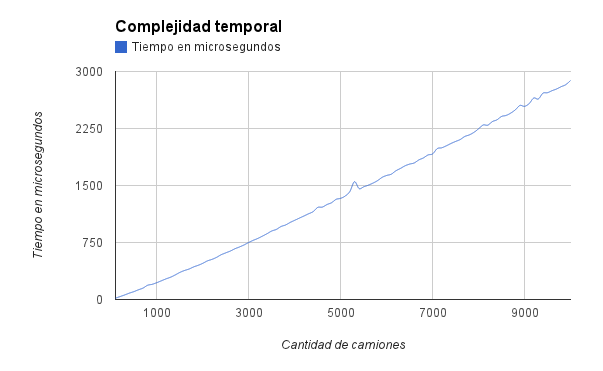
\includegraphics[scale=0.6]{images/ej1_fx.png}
\end{center}

Luego del primer grafico obtenido, decidimos graficar los pares $(x, \frac{f(x)}{x})$ con el objetivo de obtener un gr\'afico consistente con una funcion logaritmica, el resultado es el esperado, se puede observar un comportamiento logar\'itmico en el crecimiento de la funcion graficada. Notemos ademas, la imagen de la funcion resultante, esta acotada en el intervalo $\left[ 0.18 \dots 0.30\right]$, con lo cual, una funcion lineal multiplicada por valores en este intervalo, no se ver\'a alterada en exceso, explicando el grafico original obtenido en la medici\'on.
\begin{center}
	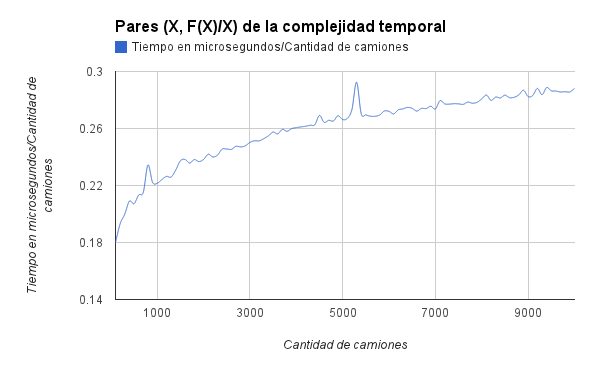
\includegraphics[scale=0.6]{images/ej1_fx_x.png}
	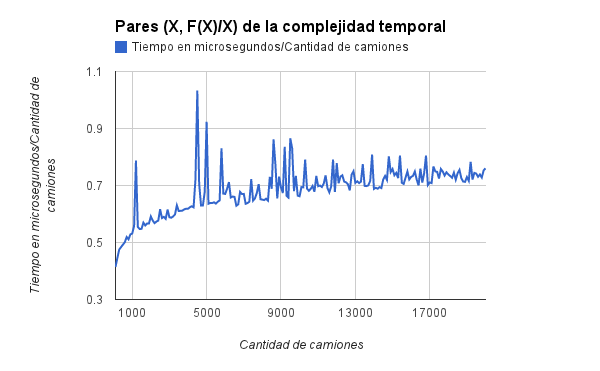
\includegraphics[scale=0.6]{images/ej1_fx_x_bis.png}
\end{center}

Como medida adicional, tambien graficamos los pares $(x, \frac{f(x)}{Log(x)})$ para tener una mayor certeza acerca de la funcion inicial. Podemos observar una funcion que es una escala de la funci\'on original, lo cual tiene sentido, dado el intervalo acotado del logaritmo que acompa\~na la funcion lineal multiplicando en la expresi\'on  \textbf{junto a una constante positiva menor que uno}. Probamos en dos casos, uno con una gran amplitud en en el intervalo de generacion de numeros aleatorios para los dias de la entrada, y otro con una amplitud m\'as limitada, el resultado fue el mismo en todos los gr\'aficos salvo en el logaritmico, lo cual puede explicarse por la busqueda binaria que se realiza sobre el conjunto de tuplas ordenadas (Dia, Cantidad de camiones hasta ese dia), lo cual tiene una complejidad O(k.logk) donde k = \#\{Cantidad de dias distintos en la entrada\}
\begin{center}
	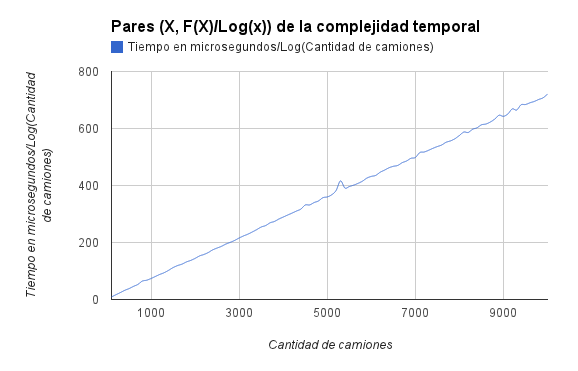
\includegraphics[scale=0.6]{images/ej1_fx_logx.png}
\end{center}

Finalmente graficamos los pares $(x, \frac{f(x)}{x*Log(x)})$ para constatar que se obtendr\'ia una constante, vamos que en realidad la funci\'on fluctua, pero dentro de un intervalo muy peque\~no $\left[ 0.07 \dots 0.09\right]$, lo cual consideramos es aceptable para asegurar que es una constante.

\begin{center}
	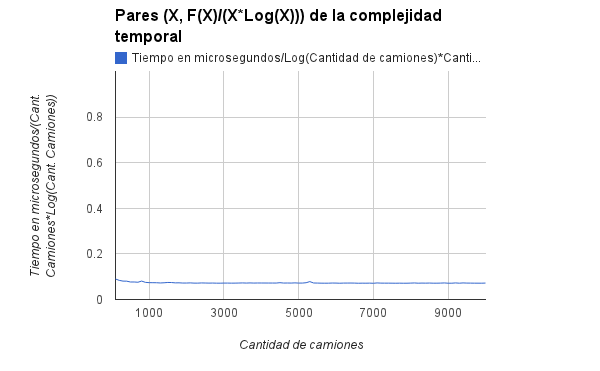
\includegraphics[scale=0.6]{images/ej1_fx_xlogx.png}
\end{center}

Como conclusi\'on podemos asegurar que el algoritmo tiene realmente la complejidad te\'orica esperada.


\subsubsection{Caso Promedio}

Para el caso promedio simplemente probamos varias intancias generadas aleatoriamente

\subsubsection{Mejor Caso}

Luego de analizar nuestro algoritmo consideramos que el mejor caso posible se da cuando el vector de entrada posee todos sus elementos iguales, es decir, todos los camiones llegan el mismo d\'ia. El ordenamiento que realiza nuestro algoritmo al comenzar se llama $introsort$, de la librer\'ia de C++, que comienza con quicksort, cambia a heapsort cuando la cantidad de llamadas recursivas excede $2*log_2(n)$. En un array de elementos iguales, la perfomance del Quicksort va a ser $(n log n)$, ya que el pivote que va a tomar en cada una de las iteraciones va a ser exactamente la mediana, causando que los dos \'indices del ciclo se unan exactamente en el medio, dividiendo los dos subproblemas en exactamente la mitad de tamano.

\vspace{2mm}

Vemos dr\'asticamente una mejora en la perfomance en la segunda parte del algoritmo. En la funci\'on que agrupa y acumula, al ser todos los elementos id\'enticos, el vector tablaDiaCantidad va a tener un solo elemento, la tupla $<unico \: elemento, longitud\_entrada>$. Por lo cual el ciclo principal del algoritmo va a realizar s\'olo una iteraci\'on hasta encontrar el intervalo \'optimo, que es el \'unico posible, el que comienza con el \'unico d\'ia en que llegan todos los camiones.

\subsubsection{Peor Caso}

No pudimos encontrar la implementaci\'on del introsort, por lo cual no sabemos qu\'e' m\'etodo utiliza para tomar el pivote. Por lo cual no sabemos cu\'al es el peor caso de este ordenamiento. De todas formas al tener complejidad $O(nlogn)$ para cualquier caso posible, la disposici\'on de los enteros del vector de entrada no influye demasiado. Busquemos peor caso de la segunda parte del algoritmo. Acto seguido del ordenamiento nuestro algoritmo recorre 1 vez el vector de entrada agrupando repetidos y acumulando. Esto es siempre linea, va a iterar una vez por cada elemento siempre, pero el peor caso posible del algoritmo debe tener todos los d\'ias de entrada distintos, as\'i esta reducci\'on efectivamente no reduce nada, y el vector resultante tablaDiaCantidad sigue siendo de longitud $n$.



\vspace{2mm}

El ciclo principal de nuestro algoritmo recorre una vez el vector tablaDiaCantidad. Por cada iteraci\'on realiza una b\'usqueda binaria. El peor caso de la b\'usqueda binaria es cuando el n\'umero a buscar no se encuentra en el arreglo. Con lo cual, para cada iteraci\'on, si para cada d\'ia $inicio$, el d\'ia $inicio + D - 1$ no se encuentra en el arreglo nos aseguraremos de que la b\'usqueda realiza la mayor cantidad de pasos posibles. Adem\'as, si $D=1$, el d\'ia a buscar queda en el extremo izquierdo del intervalo a buscar, y si $D=n$, queda siempre en el extremo derecho, lo cual tambi\'en son los peores casos de la b\'usqueda binaria. Por lo cual vamos a testear dos tipos de casos. En ambos la la distribuci\'on de d\'ias es uniforme, en el primer tipo $D=1$ y para cada d\'ia $inicio$, el d\'ia $inicio + D - 1$ nunca est\'a. En el segundo tipo de caso $D$ va a ser igual a $n$, con lo cual $inicio + D - 1$ siempre va a caer afuera del arreglo.

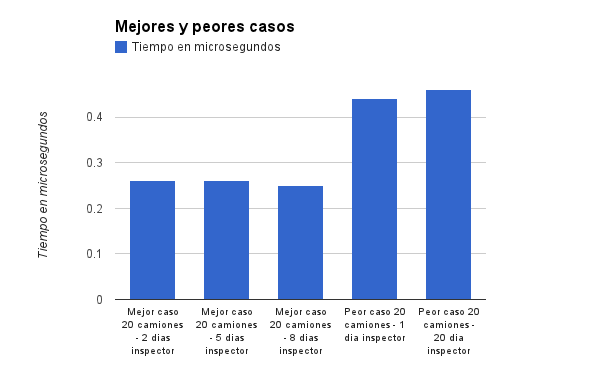
\includegraphics[scale=0.750]{images/ej1_mejor_peor.png}

\subsection{Ejercicio 2}
Para el algoritmo del ejercicio 2, tambien se observ\'o una complejidad asint\'otica te\'orica O(n.log(n)). La medici\'on de la entrada fue sobre n = \#\{ Cantidad de joyas pendientes \}. Se realiz\'o un razonamiento an\'alogo al ejercicio anterior para constatar con seguridad que se condicen las mediciones emp\'iricas con la cota te\'orica. A continuaci\'on se indican las mediciones, nuevamente graficamos la funcion original obtenida de las mediciones, dividimos sucesivamente por n, logn y finalmente nlogn obteniendo nuevamente las mismas conclusiones que en el ejercicio anterior, aunque esta vez, la funci\'on logaritmica obtenida en los pares $(x, \frac{f(x)}{x})$, es mas irregular y la funcion constante esta mas acotada dentro de un intervalo mas ajustado. Finalmente este ejercicio tambien posee una complejidad que condice con la hallada teoricamente.\\
Podemos indicar adem\'as que el peor y mejor caso de este algoritmo depende fuertemente de la implementaci\'on del algoritmo de ordenamiento de la librer\'ia de $C++$ ya que el resto del algoritmo es lineal y muy simple como para interferir con casos particulares.

\begin{center}
	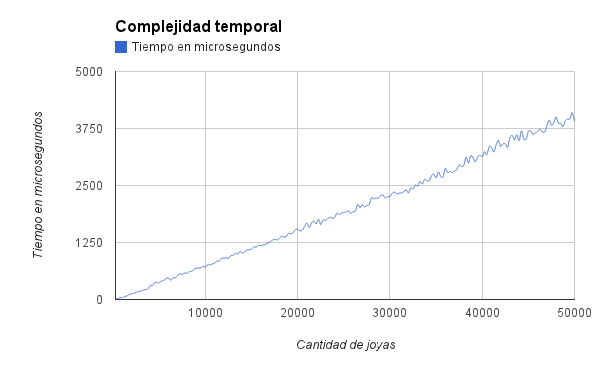
\includegraphics[scale=0.60]{images/ej2_fx.png}
	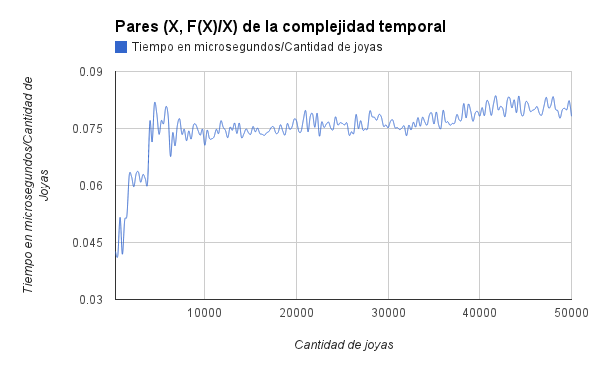
\includegraphics[scale=0.60]{images/ej2_fx_x.png}
\end{center}

\begin{center}
	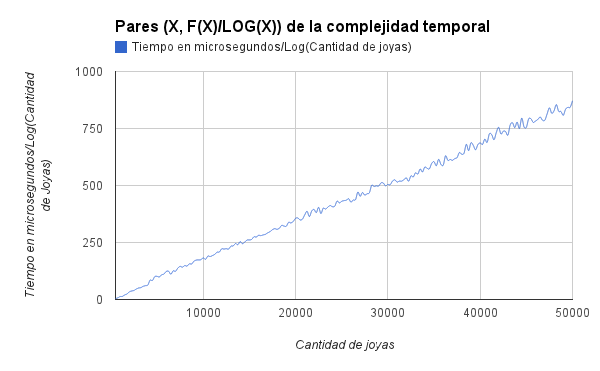
\includegraphics[scale=0.60]{images/ej2_fx_logx.png}
	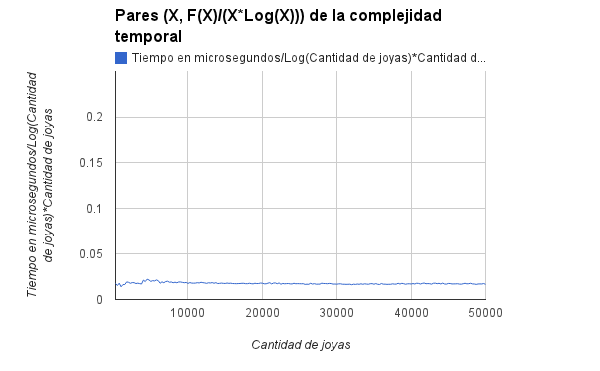
\includegraphics[scale=0.60]{images/ej2_fx_xlogx.png}
\end{center}

\subsection{Ejercicio 3} \label{mediciones_3}

Con el caso del ejercicio 3, como la complejidad es muy grande, no se pudieron realizar muchos casos de prueba con valores grandes de la entrada.

Se plante\'o como mejor caso el caso en que todas las fichas est\'en ordenadas de la forma que deben ser colocadas (o bien que todas las fichas tengan todos los lados del mismo color), por lo que encuentra el m\'aximo en $n*m$ como se explic\'o en la secci\'on \ref{ej_3:cota}, y se teste\'o dicho caso.

Tambi\'en se plante\'o como peor caso el que la poda no se realize y que pruebe la mayor cantidad de combinaciones posibles. Para lograr la mayor cantidad de combinaciones v\'alidas todas las fichas deben poder colocarse de todas las maneras posibles entre s\'i, pero si \'esto ocurriese, ser\'ia el mejor caso porque encuentra el m\'aximo valor posible de fichas a colocar en la primera iteraci\'on, entonces para minimizar la cantidad de combinaciones que se descartan, se puede poner que s\'olo una ficha no se pueda poner junto con las otras,
por ejemplo, que todas las fichas sean totalmente verdes menos 1 que sea roja. en \'este caso el primer tablero que encuentre tendr\'a $n*m - 1$ fichas colocadas, por la poda, todas las demas combinaciones que tengan 1 o m\'as casillero vac\'ios ser\'an descartadas, por lo que tenemos en total $(n*m-1)!$ combinaciones a probar.

Gr\'afico con el taman\~no de la entrada siendo la cantidad de casilleros del tablero, y el tiempo en microsegundos, se separ\'o en 2 gr\'aficos para que se aprecien los valores con entrada m\'as chica:
\begin{center}
	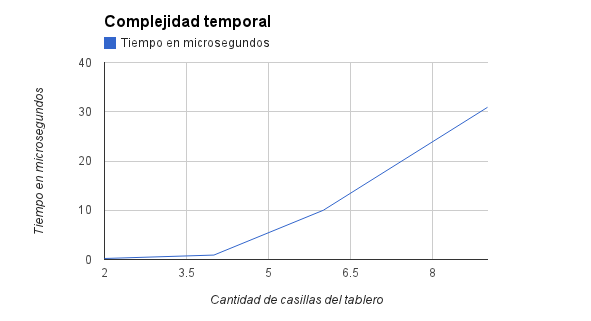
\includegraphics[scale=0.70]{images/ej3_tiempo1.png}
\end{center}
\begin{center}
	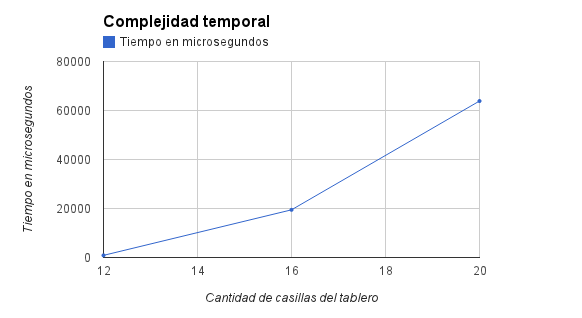
\includegraphics[scale=0.70]{images/ej3_tiempo2.png}
\end{center}

Luego se midieron los peores y mejores caso para tableros de 3x3 y 4x4 casilleros, para el peor caso de 4x4 cortamos la ejecuci\'on porque tom\'o mas de una hora y nos parecio demasiado.
\begin{center}
	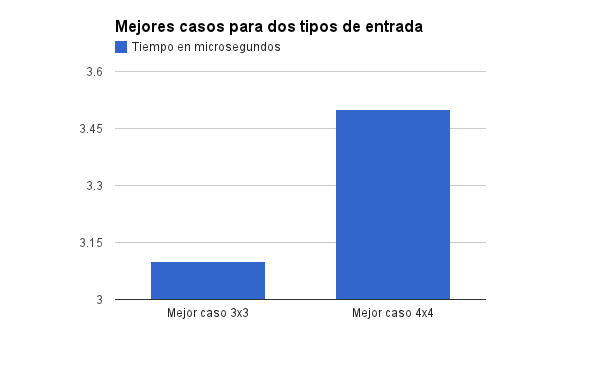
\includegraphics[scale=0.70]{images/ej3_mejor_caso.png}
	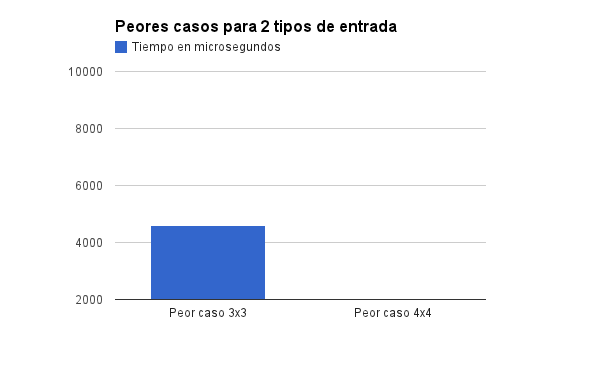
\includegraphics[scale=0.70]{images/ej3_peor_caso.png}
\end{center}

Al no poder correr una cantidad muy variada de casos con diferentes tama\~nos de la entrada, no podemos asegurar mucho sobre los gr\'aficos, de todas formas al tiempo que tard\'o cada caso, se lo dividi\'o por $(n*m)^2$ y por $(n*m)!$ para ver si la curva se llevaba a una recta
\begin{center}
	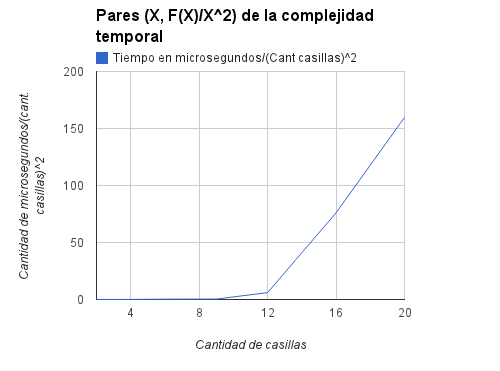
\includegraphics[scale=0.70]{images/ej3_cuadratica.png}
	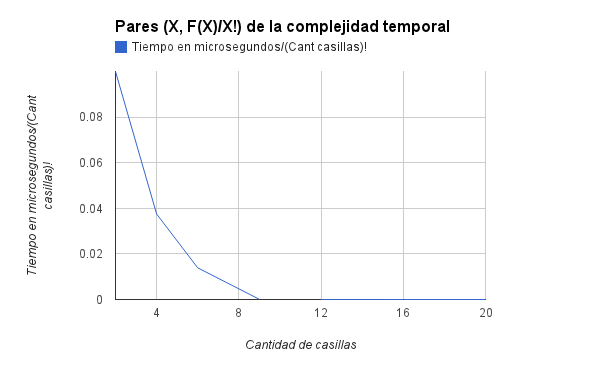
\includegraphics[scale=0.70]{images/ej3_factorial.png}
\end{center}

Como se ve, al dividir por la cuadr\'atica al menos para los primeros valores la curva a\'un est\'a creciendo, con lo cual esta no es una cota v\'alida.Asimismo cuando se divide por el factorial la curva decrece y tiende a cero, y dado que la funcion original de complejidad es creciente, podemos asegurar que la complejidad est\'a acotada por debajo por O($(n*m)^2$) y por encima por O((n*m)!) .


\section{Ap\'endice: C\'odigo fuente relevante}


\subsection{Algoritmo exacto para la resolucion de CACM}
\lstinputlisting[language=C++,tabsize=4, numbers=left, numberstyle=\tiny\color{black},mathescape=true, backgroundcolor=\color{gray}, rulecolor=\color{black}, keywordstyle=\color{blue}, commentstyle=\color{dkgreen},stringstyle=\color{mauve}, numbersep=5pt, basicstyle=\scriptsize]{codigo/exacto.cpp}

\subsection{Heuristicas constructivas golosas I: En cada paso tomar el minimo f2 dentro de las soluciones factibles(con f1 acotada)}
\lstinputlisting[language=C++,tabsize=4, numbers=left, numberstyle=\tiny\color{black},mathescape=true, backgroundcolor=\color{gray}, rulecolor=\color{black}, keywordstyle=\color{blue}, commentstyle=\color{dkgreen},stringstyle=\color{mauve}, numbersep=5pt, basicstyle=\scriptsize]{codigo/golosa1.cpp}

\subsection{Heuristicas constructivas golosas II: En cada paso tomar el minimo cociente de f1/f2 dentro de las soluciones factibles(con f1 acotada)}
\lstinputlisting[language=C++,tabsize=4, numbers=left, numberstyle=\tiny\color{black},mathescape=true, backgroundcolor=\color{gray}, rulecolor=\color{black}, keywordstyle=\color{blue}, commentstyle=\color{dkgreen},stringstyle=\color{mauve}, numbersep=5pt, basicstyle=\scriptsize]{codigo/golosa2.cpp}

\subsection{Heuristicas de busqueda local}
\lstinputlisting[language=C++,tabsize=4, numbers=left, numberstyle=\tiny\color{black},mathescape=true, backgroundcolor=\color{gray}, rulecolor=\color{black}, keywordstyle=\color{blue}, commentstyle=\color{dkgreen},stringstyle=\color{mauve}, numbersep=5pt, basicstyle=\scriptsize]{codigo/busquedalocal.cpp}

\subsection{Metaheuristica GRASP: Solucion propuesta}
\lstinputlisting[language=C++,tabsize=4, numbers=left, numberstyle=\tiny\color{black},mathescape=true, backgroundcolor=\color{gray}, rulecolor=\color{black}, keywordstyle=\color{blue}, commentstyle=\color{dkgreen},stringstyle=\color{mauve}, numbersep=5pt, basicstyle=\scriptsize]{codigo/grasp.cpp}

\section{Ap\'endice: Entregable e instrucciones de compilacion y benchmarking}
\subsection{Estructura de directorios}
%\begin{itemize}
%	\item \textbf{ej1:} Contiene el codigo fuente en java del ejercicio 1, tanto como los scripts de compilacion nativa, testeo y graficacion, casos de tests, mediciones, y graficos.
%	\item \textbf{ej2:} Contiene el codigo fuente en C++ del ejercicio 2 y su Makefile para compilar.
%	\item \textbf{ej3:} Contiene el codigo fuente en java del ejercicio 3, tanto como los scripts de compilacion nativa, testeo y graficacion, casos de tests, mediciones y graficos.
	%\item \textbf{informe:} Contiene los fuentes de latex, imagenes y codigo relevante junto al pdf del informe 
	%\item \textbf{casos:}	Contiene el programa que genera los casos del ej2
%\end{itemize}

\subsection{Compilacion y ejecucion}
%\begin{itemize}
	%\item \textbf{ej1:} Ejecutando ./compilacionNativa.sh se compila el programa, se crean y resuelven tests aleatorios tomando tiempos y se grafican en png los resultados.
	%\item \textbf{ej2:} utilizando el Makefile y corriendo el ejecutable.
	%\item \textbf{ej3:} Ejecutando ./compilacionNativa.sh se compila el programa, se crean y resuelven tests aleatorios tomando tiempos y se grafican en png los resultados.
%\end{itemize}

\subsection{Benchmarking}
%\begin{itemize}
	%\item \textbf{ej1:} pasandole el parametro --take-time $<$cant\_repeticiones$>$ se repite la ejecucion cant\_repeticiones veces tomando tiempo promedio en microsegundos . --generate-tests $<$cards number$>$ $<$randMin$>$ $<$randMax$>$ genera casos aleatorios correspondientes y los arroja por stdout.
	%\item \textbf{ej2:} Utilizando el programa especifico en la carpeta casos.
	%\item \textbf{ej1:} pasandole el parametro --take-time $<$cant\_repeticiones$>$ se repite la ejecucion cant\_repeticiones veces tomando tiempo promedio en microsegundos . --generate-tests $<$dimension$>$ $<$powerUp inicial$>$ genera casos aleatorios correspondientes y los arroja por stdout.y graficos.
%\end{itemize}

\end{document}

